\documentclass[11pt,a4paper]{article}

% Modern packages for a clean look
\usepackage[utf8]{inputenc}
\usepackage[T1]{fontenc}
\usepackage{lmodern} % Latin Modern fonts
\usepackage[margin=2.5cm]{geometry} % Page margins
\usepackage{microtype} % Improves typography
\usepackage{amsmath,amssymb,amsfonts,mathtools} % Math packages
\usepackage{xcolor} % For colors
\usepackage{graphicx} % For images
\usepackage{float} % For image placement
\usepackage{booktabs} % For nice tables
\usepackage{enumitem} % For customizing lists
\usepackage{fancyhdr} % For headers and footers
\usepackage{titlesec} % For section formatting
\usepackage{mdframed} % For nice framed boxes
\usepackage{listings} % For code blocks
\usepackage{lstfiracode} % Fira Code font for listings
\usepackage[colorlinks=true,linkcolor=blue,urlcolor=blue,citecolor=blue]{hyperref} % For hyperlinks

% Define colors
\definecolor{maincolor}{RGB}{0, 90, 160}
\definecolor{secondcolor}{RGB}{0, 130, 130}
\definecolor{codebackground}{RGB}{248, 248, 248}
\definecolor{codecomment}{RGB}{100, 100, 100}
\definecolor{codestring}{RGB}{180, 40, 40}
\definecolor{codekeyword}{RGB}{40, 40, 180}
\definecolor{warningcolor}{RGB}{180, 80, 0}
\definecolor{tipcolor}{RGB}{0, 140, 0}

% Section formatting
\titleformat{\section}
  {\color{maincolor}\normalfont\Large\bfseries}
  {\thesection}{1em}{}
\titleformat{\subsection}
  {\color{secondcolor}\normalfont\large\bfseries}
  {\thesubsection}{1em}{}
\titleformat{\subsubsection}
  {\normalfont\normalsize\bfseries}
  {\thesubsubsection}{1em}{}

% Code listing style
\lstdefinestyle{mystyle}{
    backgroundcolor=\color{codebackground},
    commentstyle=\color{codecomment},
    keywordstyle=\color{codekeyword},
    stringstyle=\color{codestring},
    basicstyle=\ttfamily\small,
    breakatwhitespace=false,
    breaklines=true,
    captionpos=b,
    keepspaces=true,
    numbersep=5pt,
    showspaces=false,
    showstringspaces=false,
    showtabs=false,
    tabsize=2,
    frame=leftline,
    framesep=5pt,
    framerule=1pt,
    rulecolor=\color{maincolor}
}
\lstset{style=mystyle}

% Create a box for notes
\newmdenv[
  linecolor=blue!75!black,
  backgroundcolor=blue!5!white,
  linewidth=0.5pt,
  topline=true,
  rightline=true,
  bottomline=true,
  leftline=true,
  innertopmargin=10pt,
  innerbottommargin=10pt,
  innerrightmargin=10pt,
  innerleftmargin=10pt,
  frametitle=\colorbox{blue!75!black}{\color{white}\bfseries Note}
]{notebox}

% Create a box for tips
\newmdenv[
  linecolor=tipcolor!75!black,
  backgroundcolor=tipcolor!5!white,
  linewidth=0.5pt,
  topline=true,
  rightline=true,
  bottomline=true,
  leftline=true,
  innertopmargin=10pt,
  innerbottommargin=10pt,
  innerrightmargin=10pt,
  innerleftmargin=10pt,
  frametitle=\colorbox{tipcolor!75!black}{\color{white}\bfseries Tip}
]{tipbox}

% Create a box for warnings
\newmdenv[
  linecolor=warningcolor!75!black,
  backgroundcolor=warningcolor!5!white,
  linewidth=0.5pt,
  topline=true,
  rightline=true,
  bottomline=true,
  leftline=true,
  innertopmargin=10pt,
  innerbottommargin=10pt,
  innerrightmargin=10pt,
  innerleftmargin=10pt,
  frametitle=\colorbox{warningcolor!75!black}{\color{white}\bfseries Warning}
]{warningbox}

% Page style
\pagestyle{fancy}
\fancyhf{}
\fancyhead[L]{\textit{Statistical Methods}}
\fancyhead[R]{\thepage}
\renewcommand{\headrulewidth}{0.4pt}
\renewcommand{\footrulewidth}{0pt}

% Document information
\title{\color{maincolor}\LARGE \textbf{Comprehensive Study Guide: Statistical Methods}}
\author{Department of Statistics}
\date{\today}

\begin{document}

\maketitle
\thispagestyle{empty}

\tableofcontents
\newpage

\section*{Introduction}
\addcontentsline{toc}{section}{Introduction}

This comprehensive study guide covers essential statistical methods for data analysis and modeling. Statistics provides the foundation for extracting meaningful insights from data, testing hypotheses, and building predictive models. The methods presented in this guide are widely used across various domains including scientific research, business analytics, machine learning, and social sciences.

\begin{notebox}
This guide assumes a basic understanding of probability theory and calculus. For each statistical method, we provide both the theoretical foundation and practical implementation in R, along with visualizations to enhance understanding.
\end{notebox}

As you work through this guide, focus on developing both conceptual understanding and practical application skills. The included R code examples can be adapted to your specific datasets and research questions.

\section{Hypothesis Testing}

Hypothesis testing is a fundamental statistical approach used to determine whether an observed difference is statistically significant or merely due to random variation. This systematic procedure allows researchers to make evidence-based decisions by evaluating claims about population parameters.

\begin{tipbox}
Before conducting any hypothesis test, clearly define:
\begin{itemize}
  \item Your research question
  \item Null and alternative hypotheses
  \item Significance level ($\alpha$)
  \item The appropriate test statistic
\end{itemize}
\end{tipbox}

\subsection{Statistical Tests}
\subsubsection{Student's t-test}

\paragraph{One Sample t-test}  
The one-sample t-test evaluates whether the mean of a sample differs from a specified value. This test is particularly useful when working with small samples from normally distributed populations.

\subparagraph{Mathematical Framework:}  

Consider a sample $X_1, X_2, \ldots, X_n$ of independent observations following a normal distribution $N(\mu, \sigma^2)$. To test $H_0: \mu = \mu_0$ versus $H_1: \mu \neq \mu_0$ (two-sided) or $H_0: \mu \leq \mu_0$ versus $H_1: \mu > \mu_0$ (one-sided), we compute the test statistic:
\begin{equation}
T_{stat} = \frac{\bar{X} - \mu_0}{S/\sqrt{n}}
\end{equation}
where:
\begin{itemize}
  \item $\bar{X} = \frac{1}{n}\sum_{i=1}^n X_i$ is the sample mean
  \item $S^2 = \frac{1}{n-1}\sum_{i=1}^n (X_i - \bar{X})^2$ is the sample variance
\end{itemize}

Under $H_0$, this statistic follows a t-distribution with $n-1$ degrees of freedom.

\paragraph{Decision Rule:}
\begin{itemize}
  \item For a two-sided test at significance level $\alpha$:
    \begin{itemize}
      \item Reject $H_0$ if $|T_{stat}| > t_{1-\alpha/2, n-1}$
      \item Reject $H_0$ if p-value $< \alpha$
    \end{itemize}
  \item For a one-sided test (greater than) at significance level $\alpha$:
    \begin{itemize}
      \item Reject $H_0$ if $T_{stat} > t_{1-\alpha, n-1}$
      \item Reject $H_0$ if p-value $< \alpha$
    \end{itemize}
\end{itemize}

\paragraph{R Implementation:}
\begin{lstlisting}[language=R]
# Manual calculation
alpha <- 0.05
x_mean <- mean(x)
x_sd <- sd(x)
n <- length(x)
df <- n - 1
t.stat <- sqrt(n)*(x_mean-mu0)/x_sd
p.value <- 1 - pt(t.stat, df)  # for one-sided (greater than)
p.value <- 2 * (1 - pt(abs(t.stat), df))  # for two-sided

# Or simply use the built-in function:
t.test(x, alternative="greater", mu=mu0)  # one-sided
t.test(x, alternative="two.sided", mu=mu0)  # two-sided
\end{lstlisting}

\begin{figure}[htb]
    \centering
    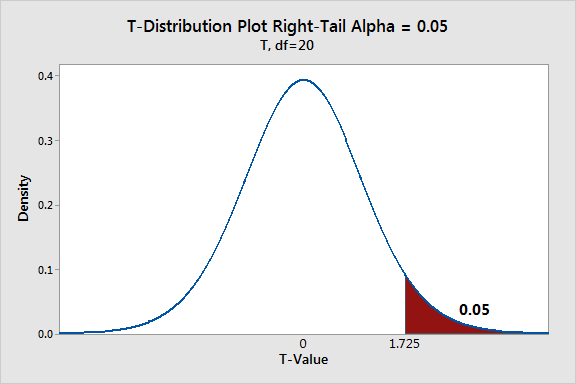
\includegraphics[width=0.8\textwidth]{t-test.png}
    \caption{t-distribution with critical regions for a one-sample t-test at $\alpha = 0.05$.}
    \label{fig:t-dist-critical}
\end{figure}

Figure \ref{fig:t-dist-critical} shows the critical regions for a one-sample t-test at the 5\% significance level.

\subsubsection{Confidence Interval for the Mean}

A confidence interval gives a range of plausible values for the population parameter. For level $1-\alpha$, the confidence interval for $\mu$ is:
\begin{equation}
CI_{1-\alpha} = \left[\bar{X} - \frac{S}{\sqrt{n}}t_{1-\alpha/2,n-1}, \bar{X} + \frac{S}{\sqrt{n}}t_{1-\alpha/2,n-1}\right]
\end{equation}
This interval has a $1-\alpha$ probability of containing the true mean $\mu$ over many samples.

\begin{warningbox}
It is incorrect to interpret this as the probability that the true mean falls within a specific interval; rather, the procedure has a $1-\alpha$ reliability over repeated samples.
\end{warningbox}

\paragraph{R Implementation:}
\begin{lstlisting}[language=R]
# Calculate 95% confidence interval
CI <- x_mean + x_sd / sqrt(n) * qt(c(alpha/2, 1-alpha/2), df)
# Or using t.test
result <- t.test(x, conf.level = 0.95)
CI <- result$conf.int
\end{lstlisting}

\begin{figure}[htb]
    \centering
    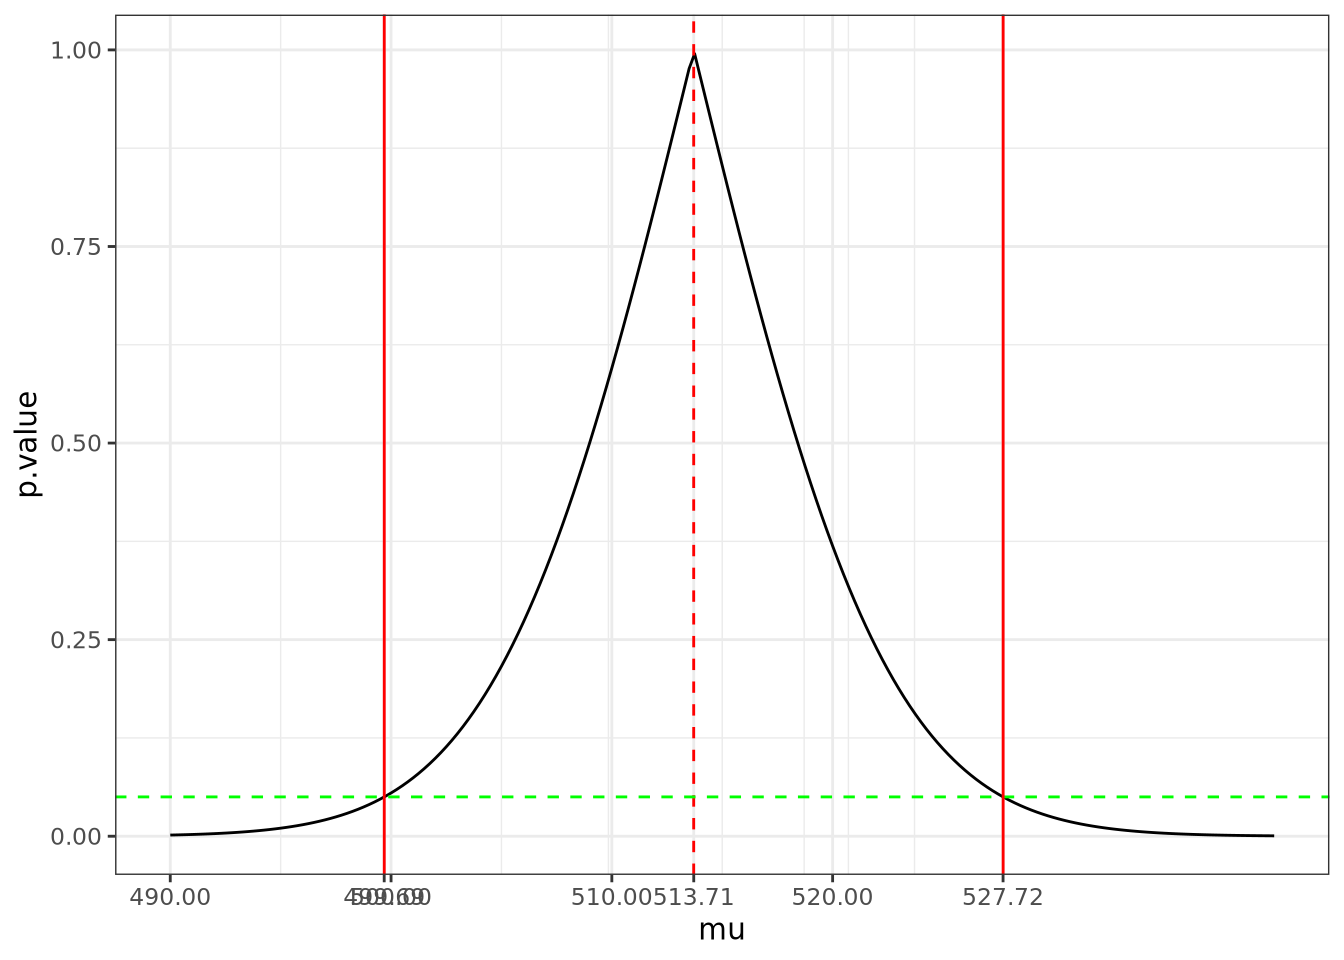
\includegraphics[width=0.6\textwidth]{confidence-intervals.png}
    \caption{Multiple 95\% confidence intervals; dashed line indicates the true parameter.}
    \label{fig:confidence-intervals}
\end{figure}

Figure \ref{fig:confidence-intervals} displays 95\% confidence intervals across samples.

\subsubsection{Two Samples t-test}

This test compares means from two independent groups.

\paragraph{Case 1: Equal Variances}
\begin{equation}
T_{stat} = \frac{\bar{X} - \bar{Y}}{S_p\sqrt{\frac{1}{n_x}+\frac{1}{n_y}}}
\end{equation}
with pooled variance
\[
S_p^2 = \frac{\sum_{i=1}^{n_x} (X_i-\bar{X})^2 + \sum_{i=1}^{n_y} (Y_i-\bar{Y})^2}{n_x+n_y-2}.
\]
Under $H_0: \mu_x = \mu_y$, $T_{stat}$ follows a t-distribution with $n_x+n_y-2$ degrees of freedom.

\paragraph{Case 2: Unequal Variances (Welch's t-test)}
\begin{equation}
T_{stat} = \frac{\bar{X} - \bar{Y}}{\sqrt{\frac{S_x^2}{n_x} + \frac{S_y^2}{n_y}}}
\end{equation}
with degrees of freedom approximated by the Welch-Satterthwaite equation.

\begin{tipbox}
Welch's t-test is recommended since it does not assume equal variances.
\end{tipbox}

\paragraph{R Implementation:}
\begin{lstlisting}[language=R]
# Equal variances t-test
t.test(x, y, var.equal = TRUE)

# Welch's t-test (default in R)
t.test(x, y)

# Formula interface
t.test(value ~ group, data = my_data, var.equal = FALSE)
\end{lstlisting}

\begin{figure}[htb]
    \centering
    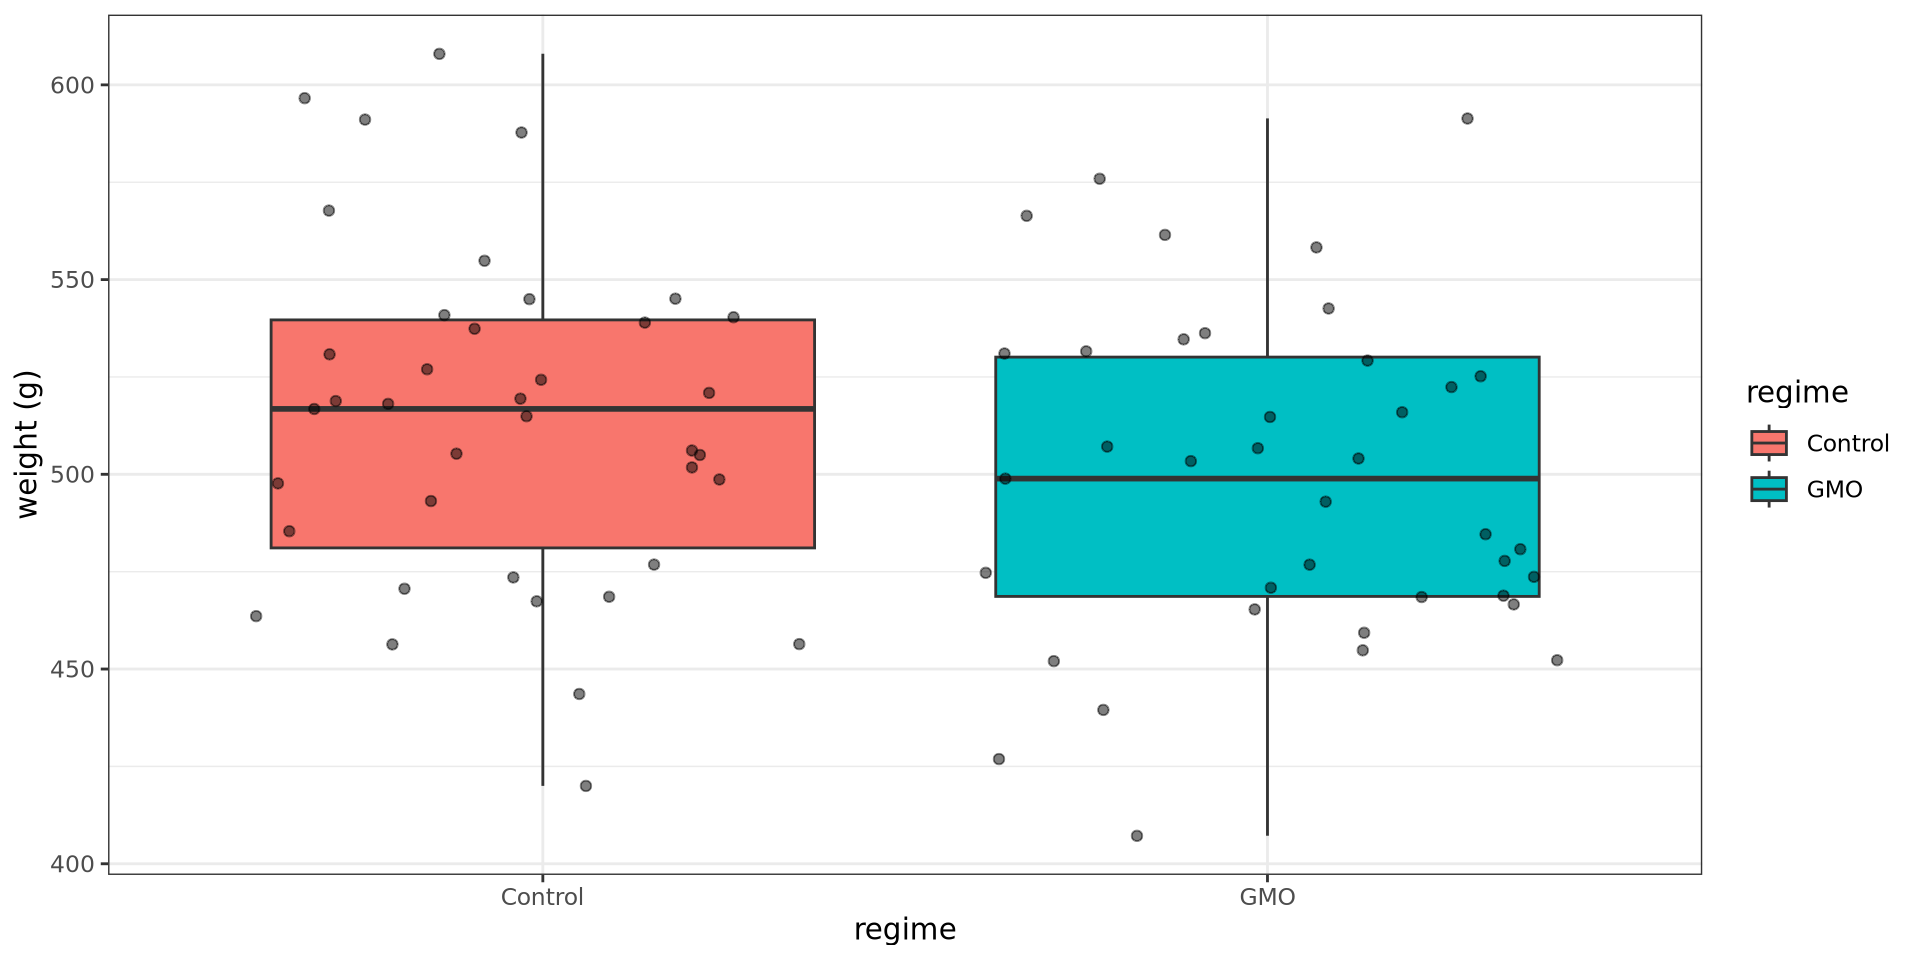
\includegraphics[width=0.8\textwidth]{group-comparison-boxplot.png}
    \caption{Boxplot comparison of two groups for central tendency and dispersion.}
    \label{fig:group-comparison}
\end{figure}

Figure \ref{fig:group-comparison} provides a visual comparison of two groups.

\subsubsection{Power of a t-test}

Power analysis helps determine the likelihood of detecting a true effect.
\begin{itemize}
  \item Effect size: $d = \frac{|\mu_x - \mu_y|}{\sigma}$
  \item Sample sizes $n_x$ and $n_y$, significance level $\alpha$, and test type (one- or two-sided)
\end{itemize}

\begin{warningbox}
Interpret non-significant results with caution if the study is underpowered.
\end{warningbox}

\paragraph{R Implementation:}
\begin{lstlisting}[language=R]
library(pwr)

# Power for specific sample size and effect size
pwr.t.test(n = 80, d = 0.3333, sig.level = 0.05, type = "two.sample", alternative = "two.sided")

# Required sample size for 80% power
pwr.t.test(power = 0.8, d = 0.3333, sig.level = 0.05, type = "two.sample", alternative = "two.sided")

# Minimum detectable effect size
pwr.t.test(n = 80, power = 0.8, sig.level = 0.05, type = "two.sample", alternative = "two.sided")
\end{lstlisting}

\begin{figure}[htb]
    \centering
    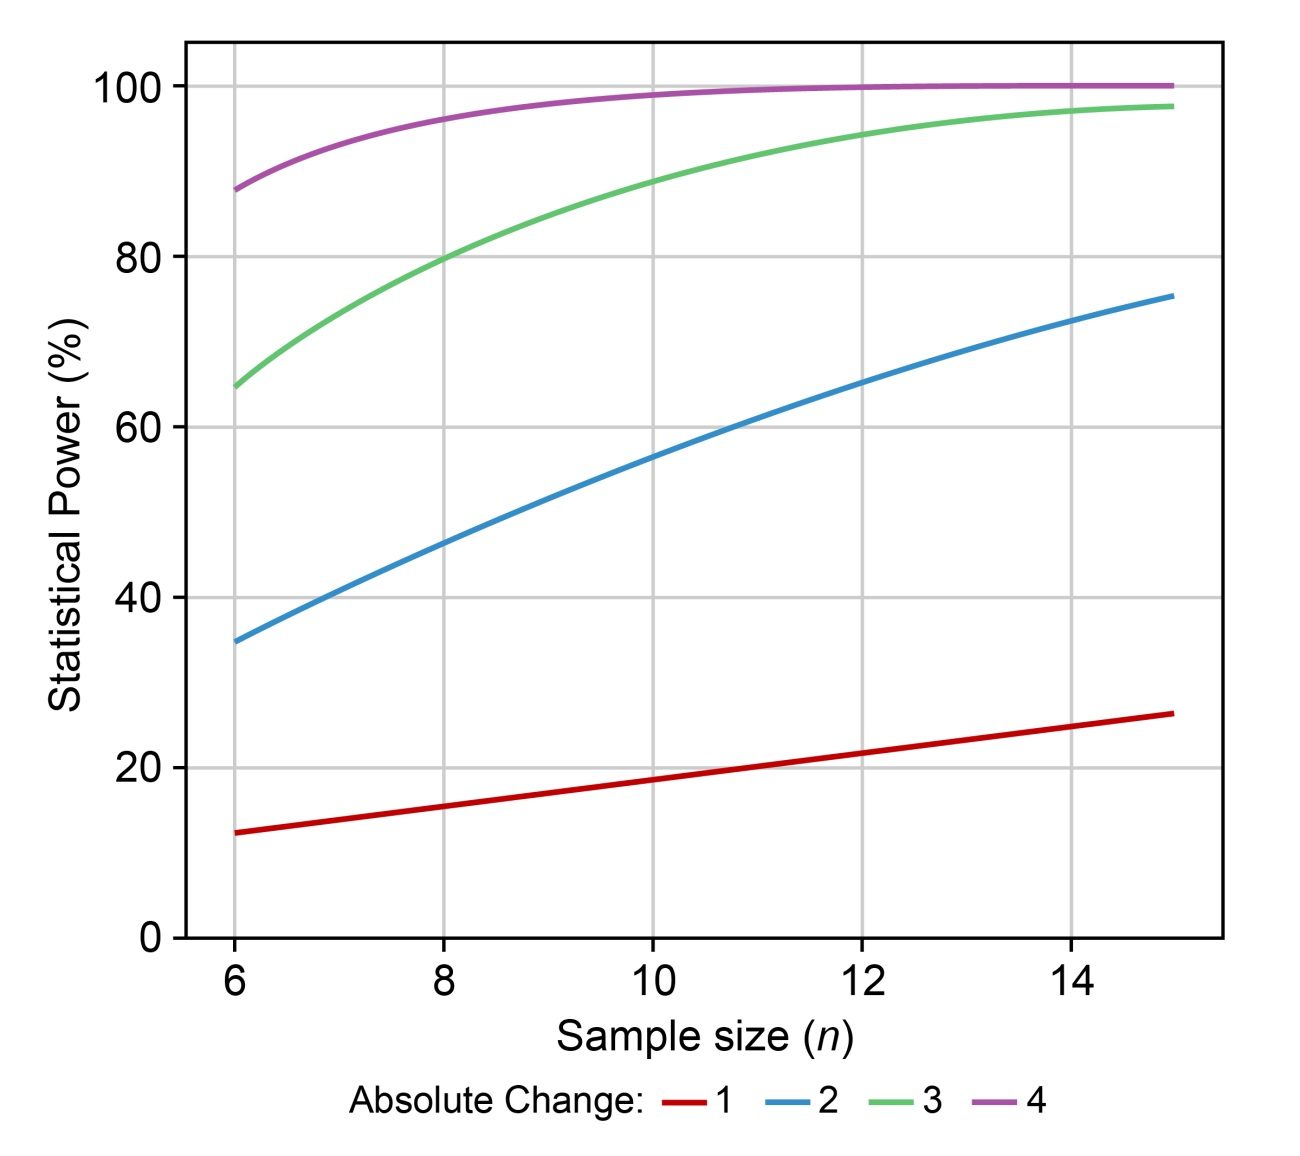
\includegraphics[width=0.6\textwidth]{power-curve.png}
    \caption{Power curves illustrating the relationship between sample size and power for various effect sizes.}
    \label{fig:power-curve}
\end{figure}

Figure \ref{fig:power-curve} shows how power increases with sample size.

\subsubsection{Wilcoxon Test}

A non-parametric alternative for small or non-normal samples.
\begin{notebox}
Use the Wilcoxon test when:
\begin{itemize}
  \item Sample sizes are small
  \item Data are non-normal or ordinal
  \item Outliers are present
\end{itemize}
\end{notebox}

\paragraph{R Implementation:}
\begin{lstlisting}[language=R]
# One-sample test (comparing to a median)
wilcox.test(x, mu = 0, alternative = "two.sided")

# Two-sample test
wilcox.test(x, y, alternative = "two.sided")

# Formula interface
wilcox.test(value ~ group, data = my_data)
\end{lstlisting}

\begin{figure}[htb]
    \centering
    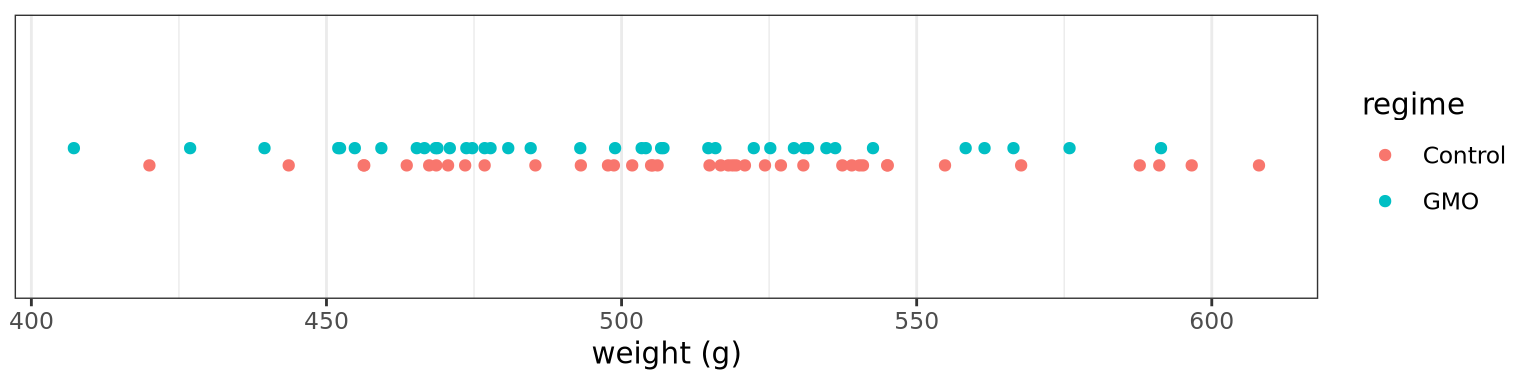
\includegraphics[width=0.8\textwidth]{wilcoxon-ranked.png}
    \caption{Rank-based comparison in the Wilcoxon test, illustrating robust ordering of values.}
    \label{fig:rank-comparison}
\end{figure}

Figure \ref{fig:rank-comparison} highlights the rank-based nature of the Wilcoxon test.

\subsection{Multiple Testing}

Multiple testing increases the risk of false positives; corrections are necessary.

\subsubsection{The Multiple Testing Problem}

Without correction, the chance of false positives increases with the number of tests.
\begin{figure}[htb]
    \centering
    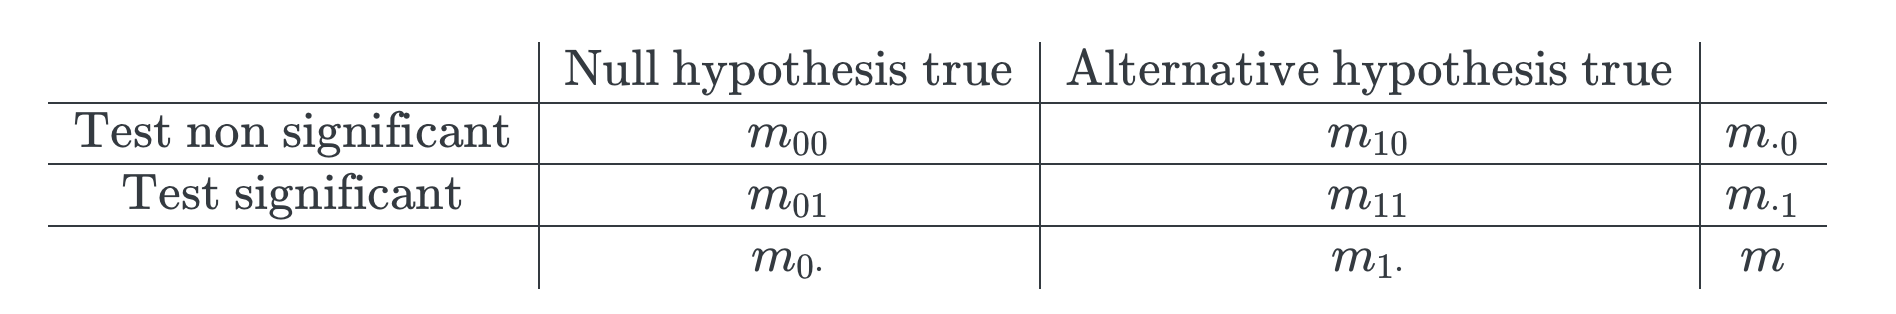
\includegraphics[width=0.8\textwidth]{false-pos-example.png}
    \caption{Illustration of false positives increasing with multiple tests.}
    \label{fig:multiple-testing}
\end{figure}

Figure \ref{fig:multiple-testing} shows this effect.

\subsubsection{Key Metrics}
\begin{itemize}
  \item \textbf{FWER:} Probability of at least one false positive.
  \item \textbf{FDR:} Expected proportion of false positives among discoveries.
\end{itemize}

\subsubsection{Bonferroni Correction}
\begin{lstlisting}[language=R]
p_adjusted <- p.adjust(p_values, method = "bonferroni")
p_adjusted <- pmin(p_values * m, 1)
\end{lstlisting}

\subsubsection{Benjamini-Yekutieli (BY) and Benjamini-Hochberg (BH) Procedures}
\begin{lstlisting}[language=R]
# BH correction
p_adjusted <- p.adjust(p_values, method = "BH")

# BY correction
p_adjusted <- p.adjust(p_values, method = "BY")

# Compare methods
p_adjusted_all <- sapply(c("bonferroni", "holm", "hochberg", "BH", "BY"), function(method) p.adjust(p_values, method))
\end{lstlisting}

\begin{figure}[htb]
    \centering
    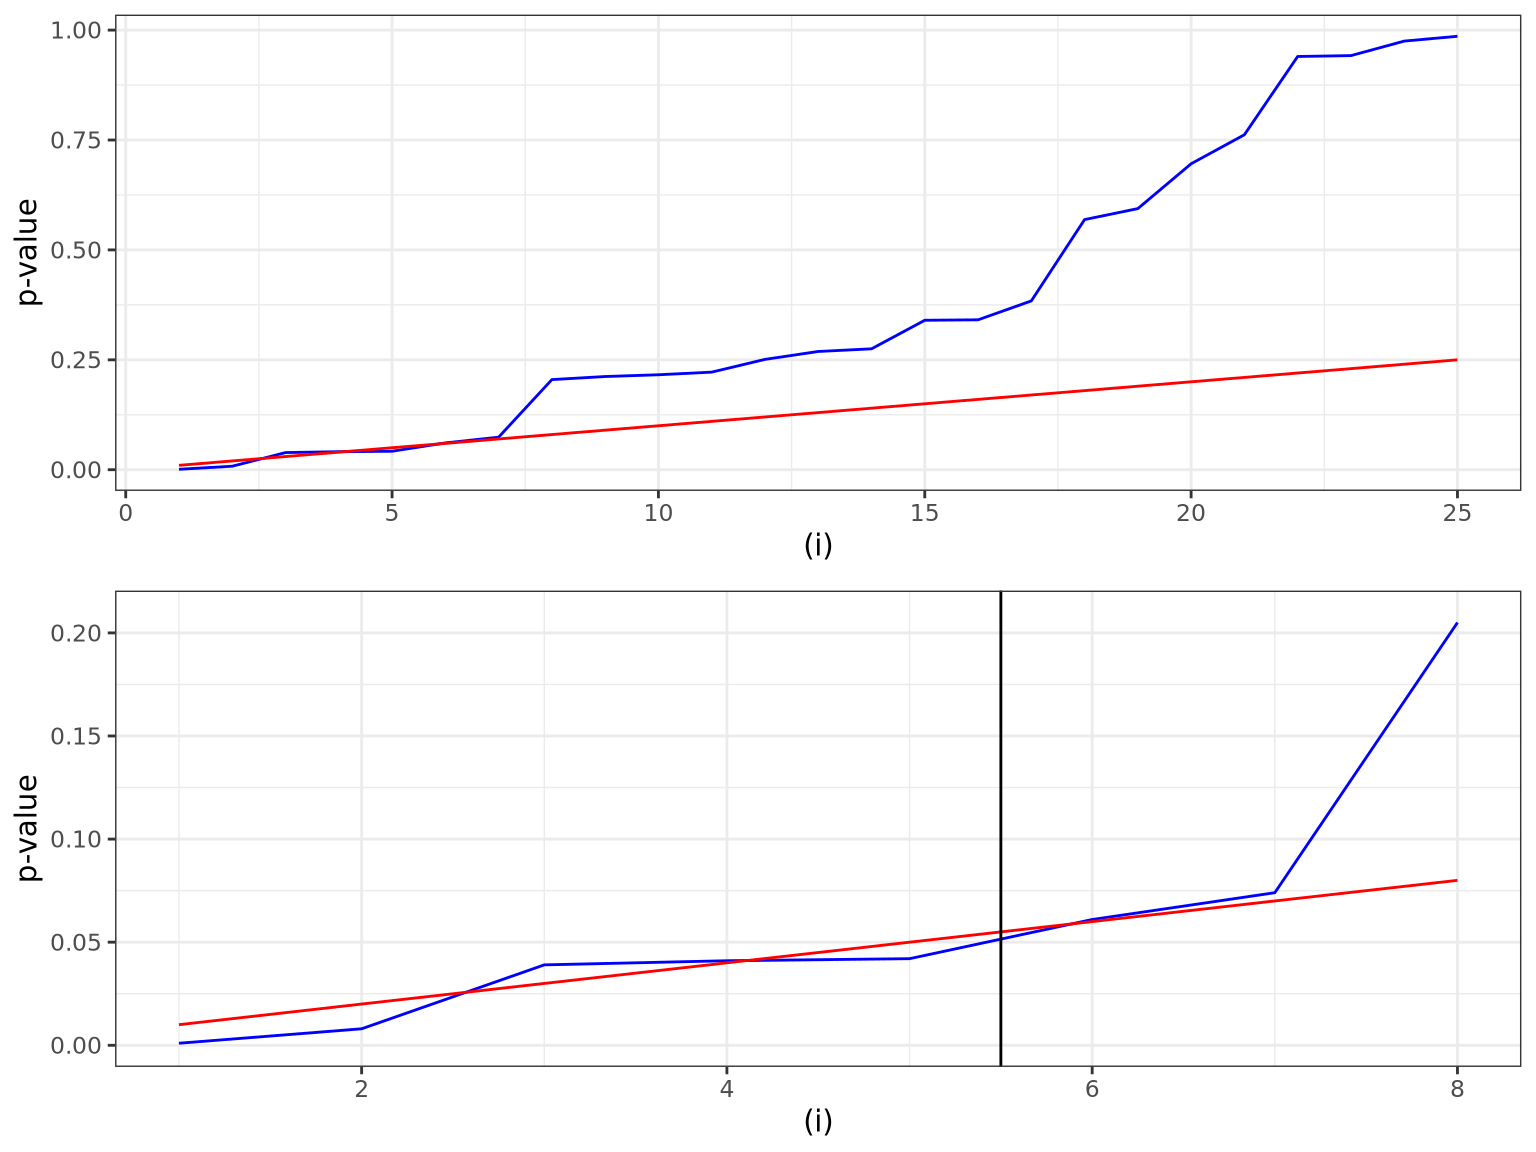
\includegraphics[width=0.8\textwidth]{multiple-testing-problem.png}
    \caption{Ordered p-values with Bonferroni and BH thresholds.}
    \label{fig:p-value-thresholds}
\end{figure}

Figure \ref{fig:p-value-thresholds} compares correction thresholds.

\subsubsection{Holm's Procedure}
\begin{lstlisting}[language=R]
p_adjusted <- p.adjust(p_values, method = "holm")
\end{lstlisting}

\subsubsection{Guidelines for Multiple Testing}
\begin{tipbox}
Consider research context, number of tests, dependency, and whether the research is exploratory or confirmatory when choosing a correction method.
\end{tipbox}

\newpage

\section{Regression Models}

Regression models explore relationships between variables.

\subsection{Linear Regression: Quick Recap}

\subsubsection{Model Formulation}
\begin{equation}
y_j = f(x_j, \beta) + \varepsilon_j
\end{equation}
with $f(x_j, \beta) = \beta_0 + \beta_1 x_j$ for simple linear regression.

\begin{notebox}
Assumptions:
\begin{itemize}
  \item Linearity
  \item Independence
  \item Homoscedasticity
  \item Normality of errors
\end{itemize}
\end{notebox}

\subsubsection{Ordinary Least Squares Estimation}
\begin{equation}
\hat{\beta} = (X'X)^{-1}X'y
\end{equation}

\paragraph{R Implementation:}
\begin{lstlisting}[language=R]
lm1 <- lm(dist ~ speed, data = cars)
lm2 <- lm(mpg ~ wt + hp + disp, data = mtcars)
summary(lm1)
coef(lm1)
confint(lm1)
\end{lstlisting}

\subsubsection{Parameter Inference}

Standard errors, t-statistics, p-values, and confidence intervals are derived from the variance-covariance matrix.

\begin{figure}[htb]
    \centering
    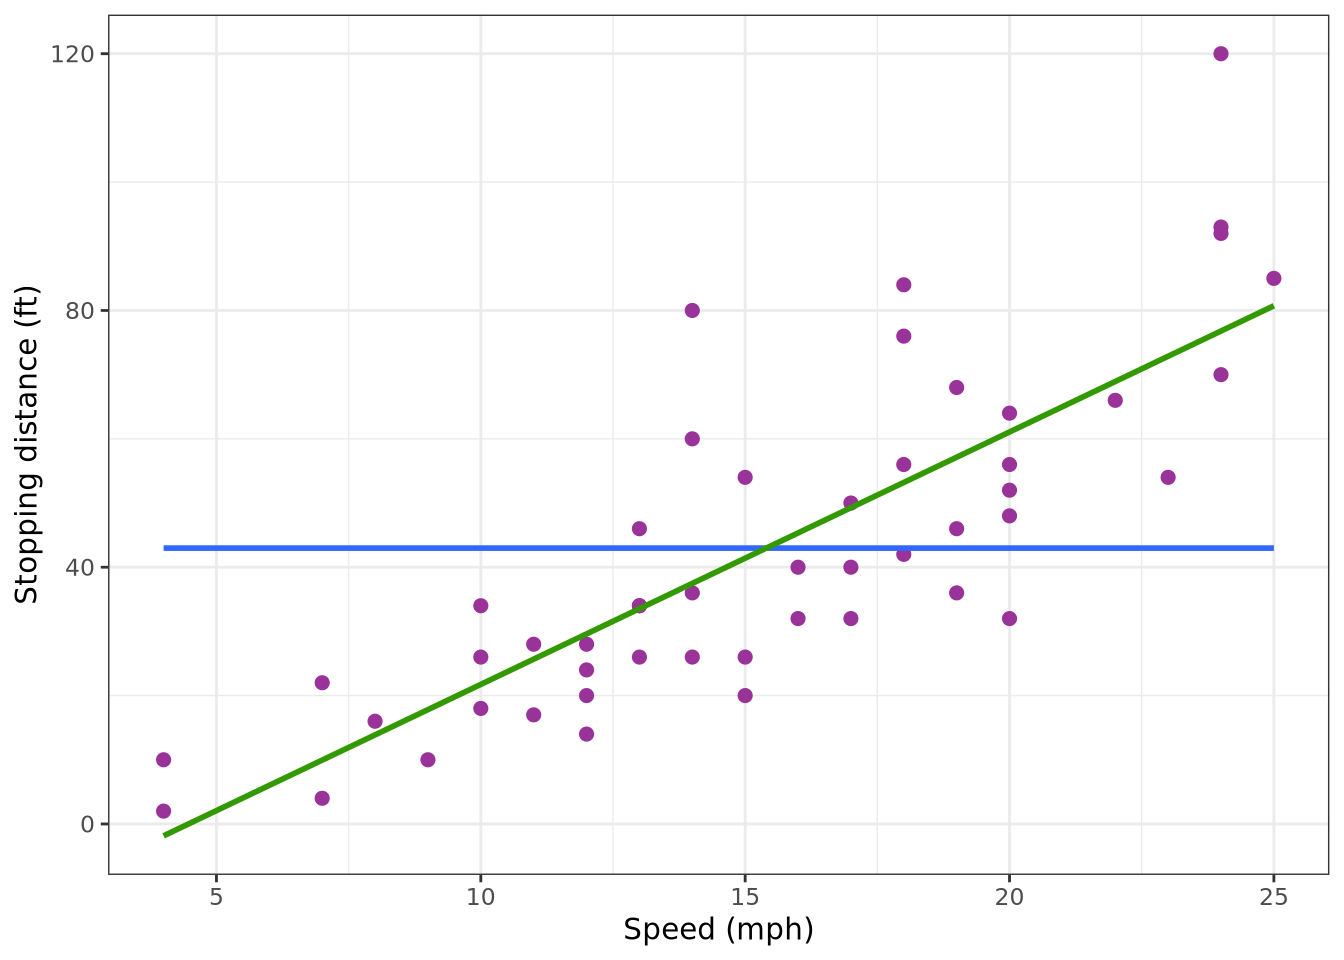
\includegraphics[width=0.8\textwidth]{regression-fit.png}
    \caption{Scatter plot with fitted regression line and residuals.}
    \label{fig:regression-fit}
\end{figure}

Figure \ref{fig:regression-fit} displays the fitted line and residuals.

\subsubsection{Model Assessment}

Metrics include R-squared, adjusted R-squared, F-statistic, and diagnostic plots.

\begin{tipbox}
Use F-tests, AIC/BIC, or cross-validation for model comparison.
\end{tipbox}

\begin{figure}[htb]
    \centering
    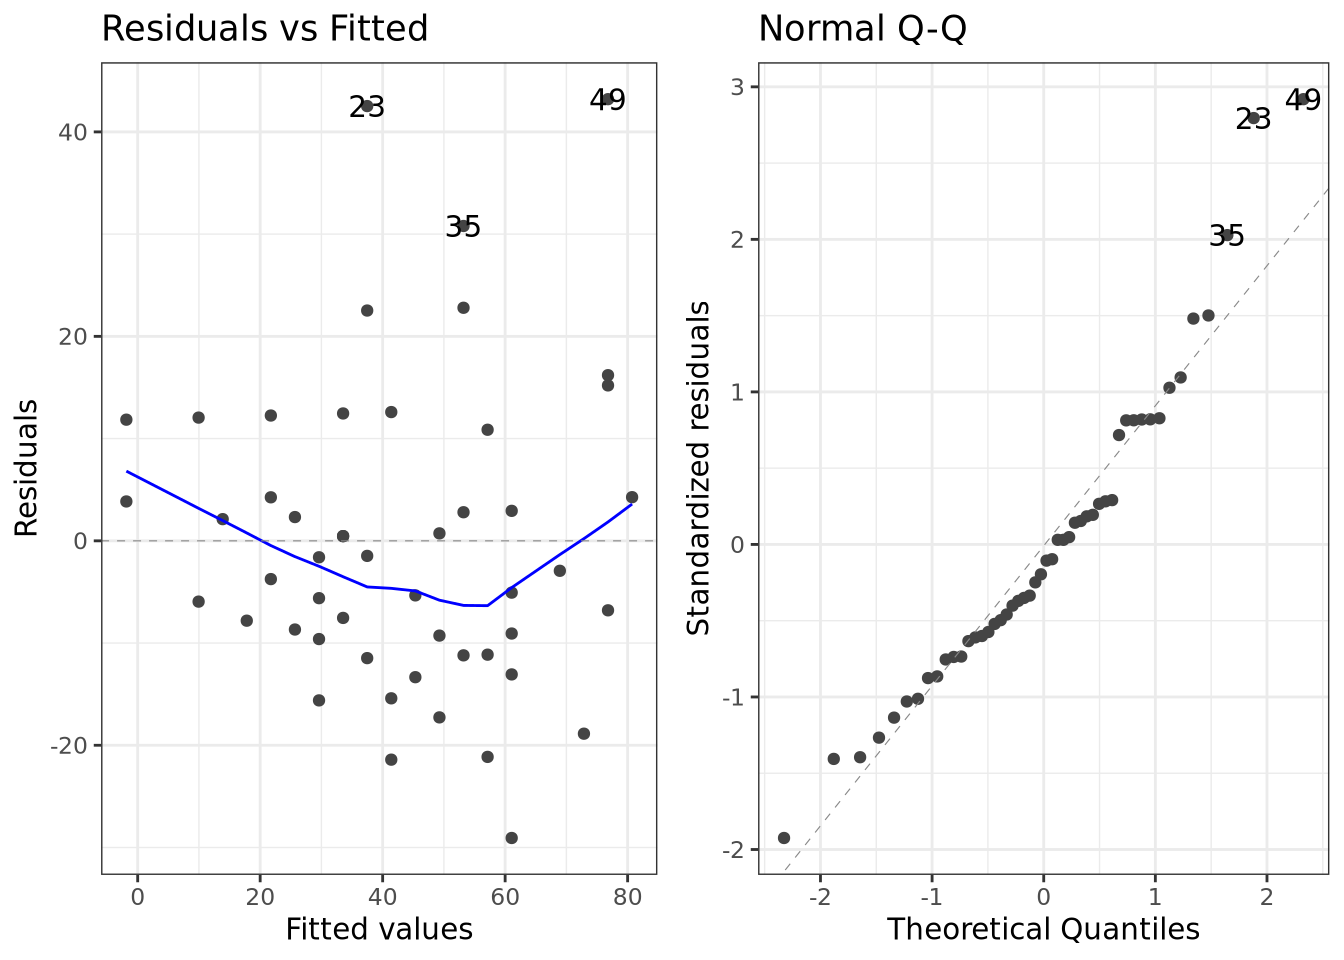
\includegraphics[width=0.8\textwidth]{diagnostic-plots.png}
    \caption{Diagnostic plots for regression model assumptions.}
    \label{fig:diagnostic-plots}
\end{figure}

\paragraph{R Implementation for Diagnostics:}
\begin{lstlisting}[language=R]
plot(lm1)
library(ggfortify)
autoplot(lm1, which = 1:4)
plot(lm1, which = 4)
n <- length(residuals(lm1))
cooks_d <- cooks.distance(lm1)
influential <- which(cooks_d > 4/n)
\end{lstlisting}

\subsection{Polynomial Regression}

\subsubsection{Model Formulation}
\begin{equation}
f(x) = \beta_0 + \beta_1x + \beta_2x^2 + \ldots + \beta_dx^d
\end{equation}

\paragraph{R Implementation:}
\begin{lstlisting}[language=R]
lm2 <- lm(dist ~ speed + I(speed^2), data = cars)
lm2_poly <- lm(dist ~ poly(speed, degree = 2), data = cars)
anova(lm1, lm2)
summary(lm2)
\end{lstlisting}

\begin{figure}[htb]
    \centering
    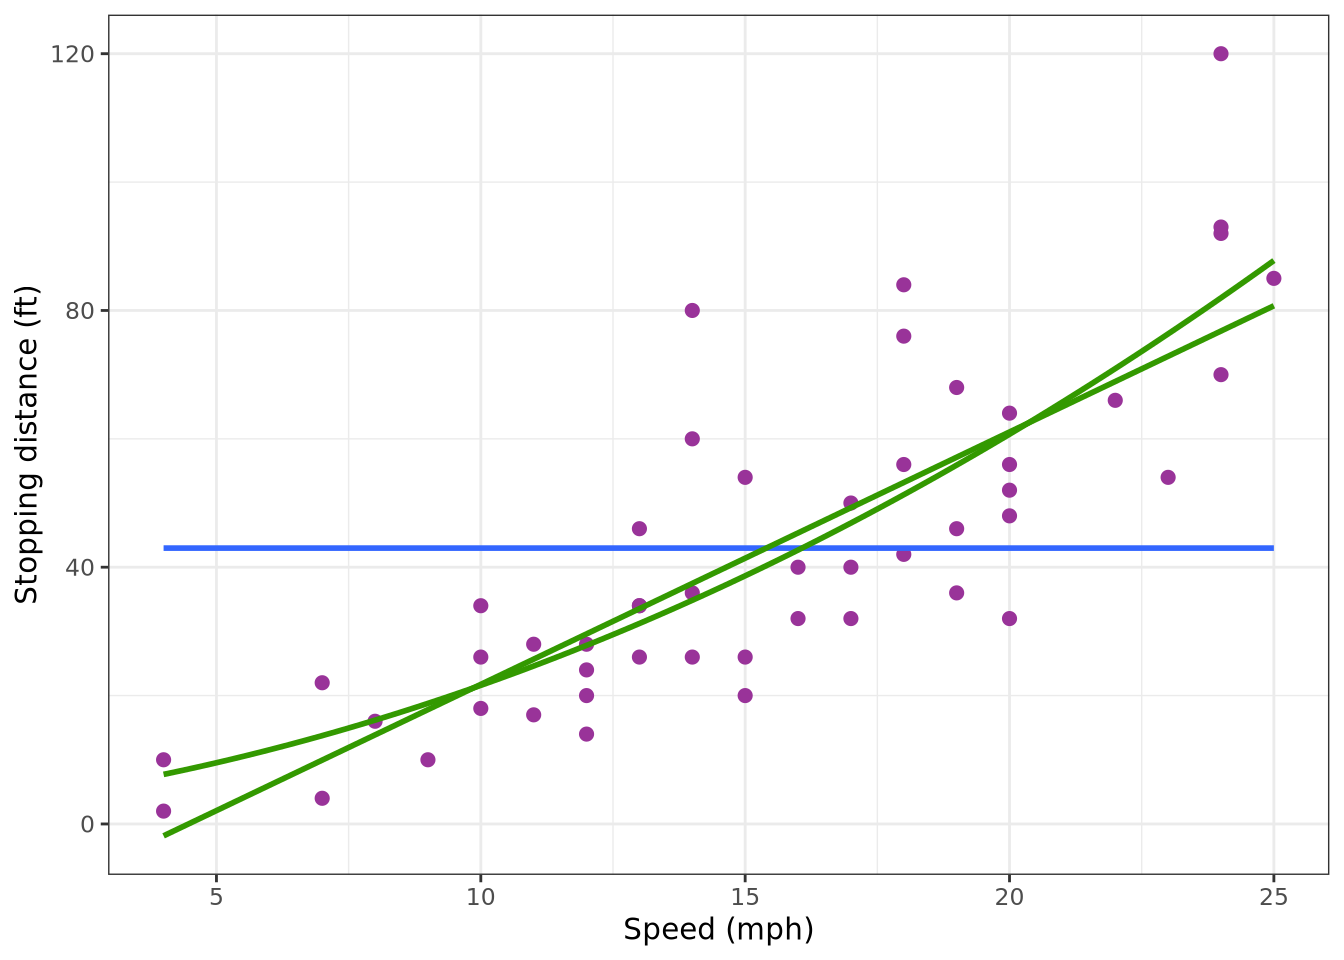
\includegraphics[width=0.8\textwidth]{polynomial-fits.png}
    \caption{Comparison of polynomial fits (linear, quadratic, cubic) on the dataset.}
    \label{fig:polynomial-fits}
\end{figure}

Figure \ref{fig:polynomial-fits} compares the different fits.

\subsubsection{Orthogonal Polynomials}
\begin{lstlisting}[language=R]
lm2_ortho <- lm(dist ~ poly(speed, degree = 2), data = cars)
lm2_raw <- lm(dist ~ poly(speed, degree = 2, raw = TRUE), data = cars)
coef(lm2_raw)
coef(lm2_ortho)
\end{lstlisting}

\begin{warningbox}
Coefficients of orthogonal polynomials are not directly interpretable.
\end{warningbox}

\subsubsection{Model Selection}
\begin{lstlisting}[language=R]
anova(lm1, lm2, lm3)
AIC(lm1, lm2, lm3)
BIC(lm1, lm2, lm3)
library(caret)
train_control <- trainControl(method = "cv", number = 10)
cv_model <- train(dist ~ poly(speed, degree = 2), data = cars, method = "lm", trControl = train_control)
\end{lstlisting}

\subsubsection{Data Transformation}
\begin{lstlisting}[language=R]
lm_loglog <- lm(log(y) ~ log(x), data = my_data)
lm_semilogy <- lm(log(y) ~ x, data = my_data)
library(MASS)
bc <- boxcox(y ~ x, data = my_data)
lambda <- bc$x[which.max(bc$y)]
\end{lstlisting}

\subsection{Nonlinear Regression}

\subsubsection{Model Examples}
\textbf{Logistic function:}
\begin{equation}
f_1(x) = \frac{A}{1 + \exp(-\gamma(x - \tau))}
\end{equation}
\textbf{Pharmacokinetic model:}
\begin{equation}
f(t, \psi) = \frac{D \cdot ka}{V(ka-ke)}\left(e^{-ke \cdot t} - e^{-ka \cdot t}\right)
\end{equation}

\begin{figure}[htb]
    \centering
    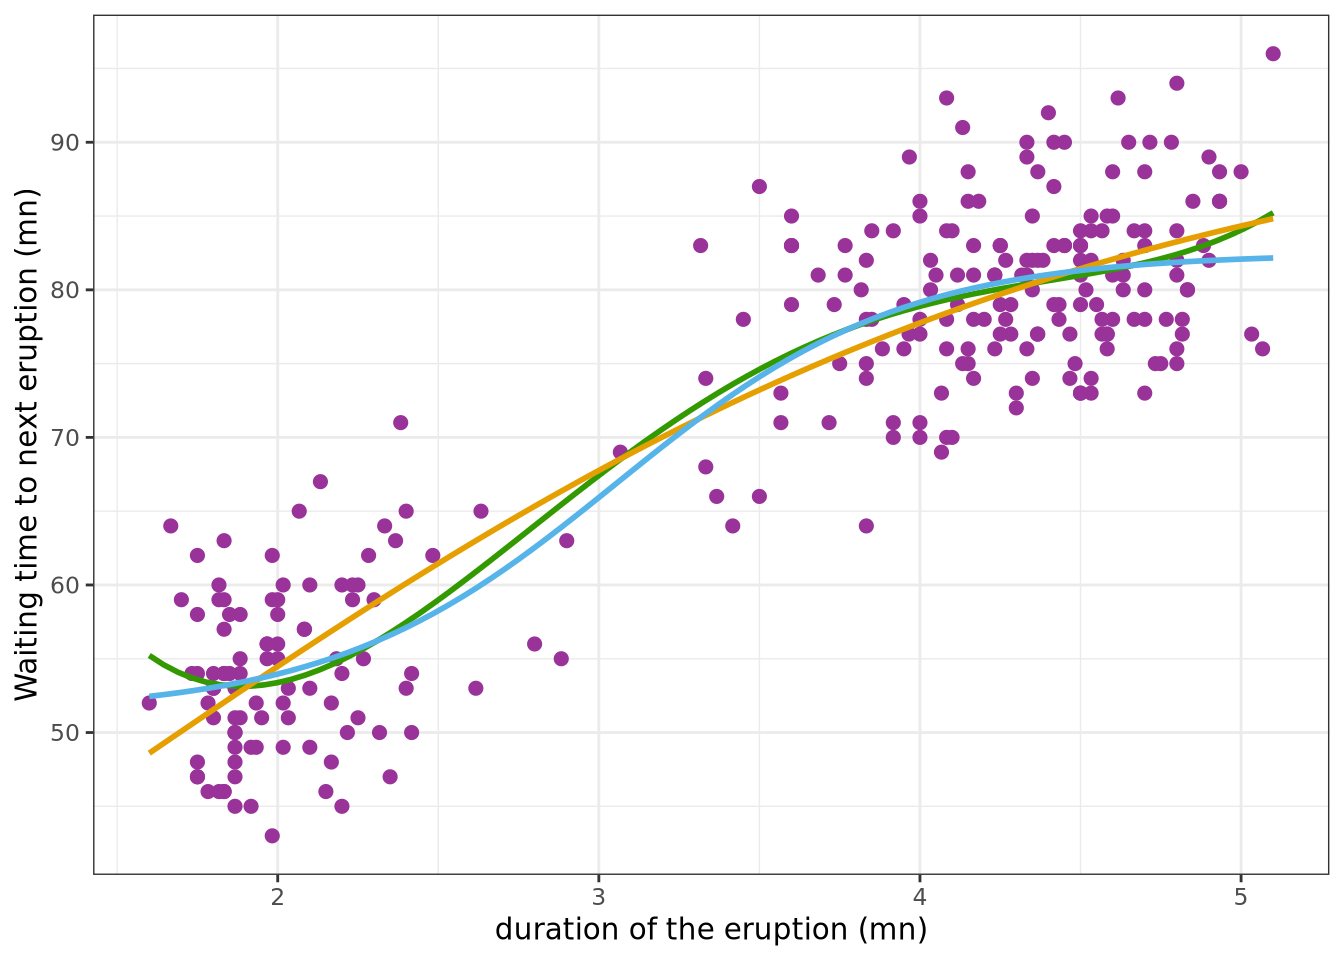
\includegraphics[width=0.8\textwidth]{nonlinear_model_curve.png}
    \caption{Nonlinear function curves for varying parameter values.}
    \label{fig:nonlinear-function}
\end{figure}

Figure \ref{fig:nonlinear-function} shows the effect of parameter changes.

\subsubsection{Parameter Estimation}
\begin{equation}
\hat{\psi} = \arg\min_{\psi} \sum_{j=1}^n (y_j - f(t_j, \psi))^2
\end{equation}

\paragraph{R Implementation:}
\begin{lstlisting}[language=R]
f1 <- function(psi, t) {
  D <- 320  
  ka <- psi[1]
  V <- psi[2]
  ke <- psi[3]
  D*ka/V/(ka-ke)*(exp(-ke*t)-exp(-ka*t))
}
model_1 <- nls(concentration ~ f1(psi, time), start = list(psi=c(ka=1, V=40, ke=0.1)), data=subject1)
summary(model_1)
confint(model_1)
\end{lstlisting}

\begin{notebox}
Nonlinear regression requires a well-specified model, good starting values, and sufficient data.
\end{notebox}

\subsubsection{Standard Error Estimation}
\begin{lstlisting}[language=R]
summary(model_1)$parameters[, "Std. Error"]
confint(model_1, level = 0.95)
library(boot)
boot_fn <- function(data, indices) {
  d <- data[indices, ]
  m <- try(nls(concentration ~ f1(psi, time), start = list(psi=coef(model_1)), data=d), silent=TRUE)
  if(inherits(m, "try-error")) return(rep(NA, 3))
  return(coef(m))
}
results <- boot(data=subject1, statistic=boot_fn, R=1000)
\end{lstlisting}

\subsubsection{Confidence and Prediction Intervals}
\begin{figure}[htb]
    \centering
    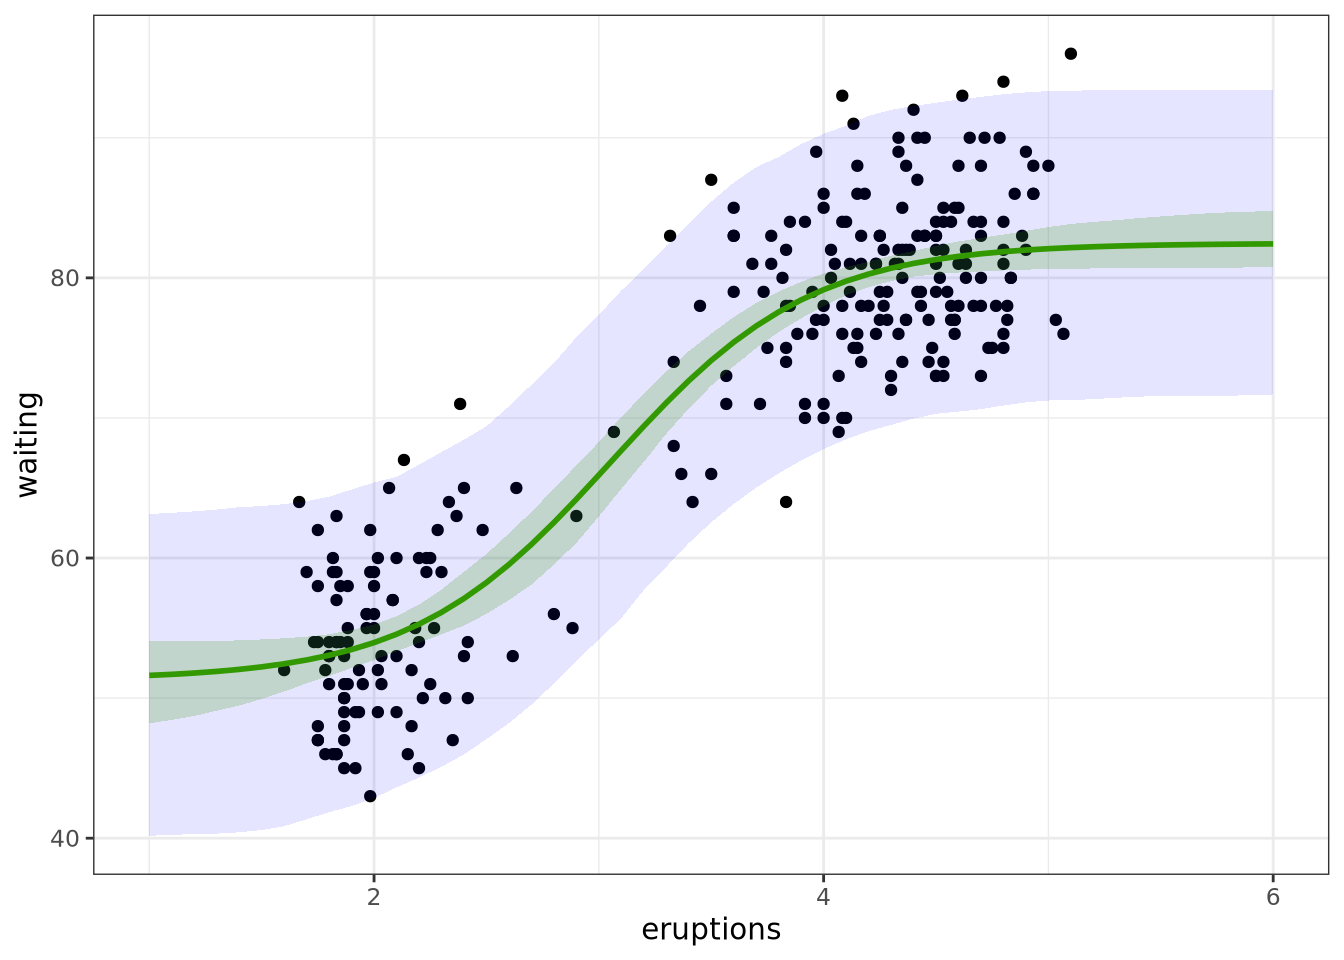
\includegraphics[width=0.8\textwidth]{confidence-prediction-bands.png}
    \caption{Nonlinear fit with confidence and prediction bands.}
    \label{fig:conf-pred-bands}
\end{figure}

\paragraph{R Implementation:}
\begin{lstlisting}[language=R]
new_data <- data.frame(time = seq(min(time), max(time), length.out = 100))
preds <- predict(model_1, newdata = new_data, se.fit = TRUE)
conf_bands <- data.frame(
  time = new_data$time,
  fit = preds$fit,
  lower = preds$fit - 1.96 * preds$se.fit,
  upper = preds$fit + 1.96 * preds$se.fit
)
sigma_hat <- summary(model_1)$sigma
pred_bands <- data.frame(
  time = new_data$time,
  fit = preds$fit,
  lower = preds$fit - 1.96 * sqrt(preds$se.fit^2 + sigma_hat^2),
  upper = preds$fit + 1.96 * sqrt(preds$se.fit^2 + sigma_hat^2)
)
\end{lstlisting}

\newpage

\section{Mixed Models}

Mixed models incorporate both fixed and random effects.

\subsection{Linear Mixed Effects Models}

\subsubsection{Model Formulation}
\begin{equation}
y_i = X_i\beta + Z_i\eta_i + \varepsilon_i
\end{equation}

\begin{tipbox}
Fixed effects correspond to factors of primary interest; random effects generalize to a larger population.
\end{tipbox}

\begin{figure}[htb]
    \centering
    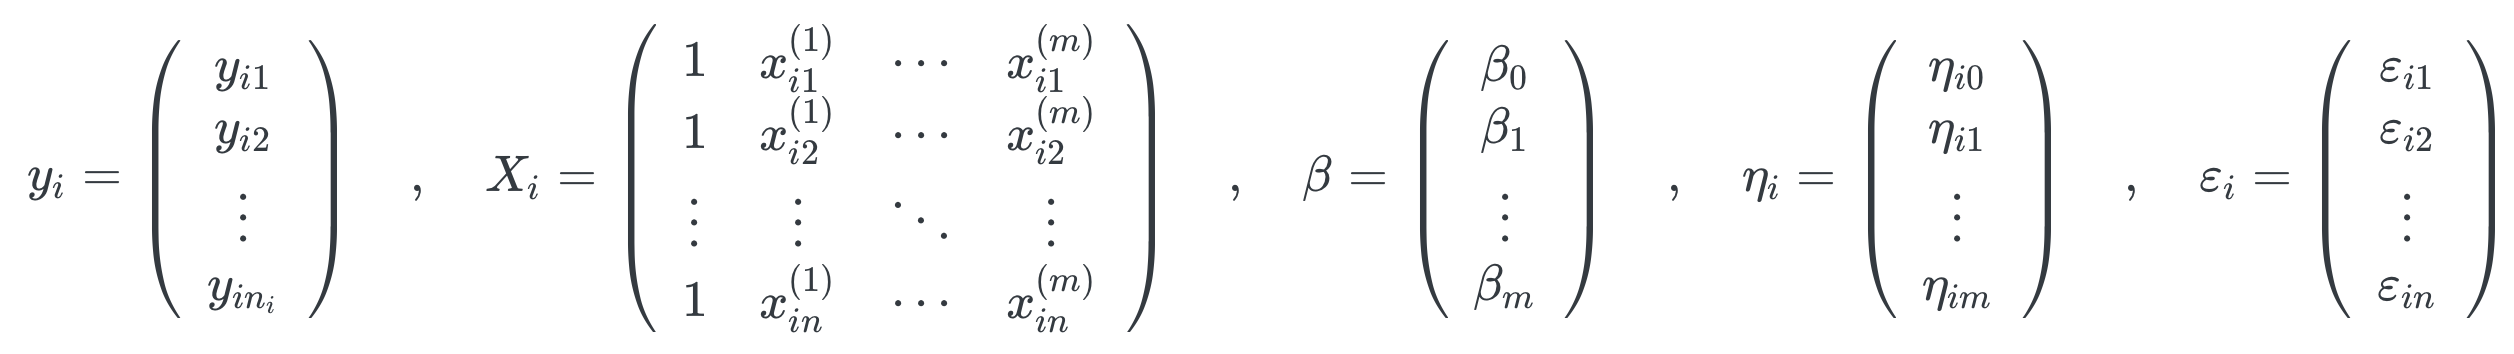
\includegraphics[width=0.8\textwidth]{hierarchical-structure.png}
    \caption{Hierarchical data structure for mixed models.}
    \label{fig:hierarchical-structure}
\end{figure}

Figure \ref{fig:hierarchical-structure} shows a typical nested data structure.

\subsubsection{Example with Orthodont Data}
\begin{figure}[htb]
    \centering
    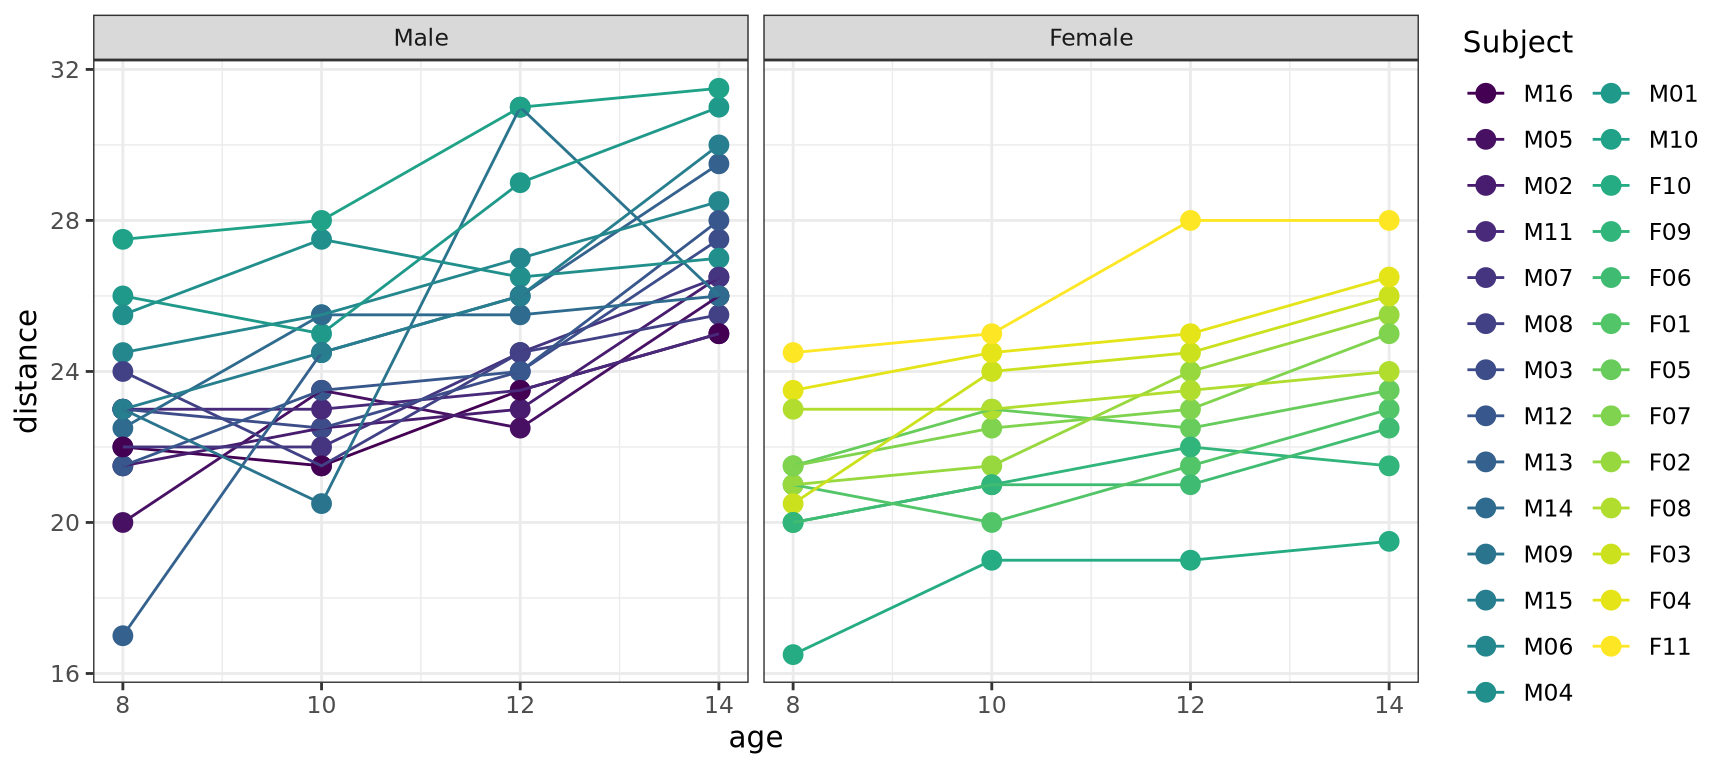
\includegraphics[width=0.8\textwidth]{orthodont-trajectories.png}
    \caption{Growth trajectories from the Orthodont dataset.}
    \label{fig:orthodont-trajectories}
\end{figure}

\paragraph{R Implementation:}
\begin{lstlisting}[language=R]
library(lme4)
lmm1 <- lmer(distance ~ age + (1|Subject), data = Orthodont)
lmm2 <- lmer(distance ~ age + (age|Subject), data = Orthodont)
lmm3 <- lmer(distance ~ age*Sex + (age|Subject), data = Orthodont)
summary(lmm2)
\end{lstlisting}

\subsubsection{Parameter Estimation}
\begin{lstlisting}[language=R]
lmm_reml <- lmer(distance ~ age + (age|Subject), data = Orthodont)
lmm_ml <- lmer(distance ~ age + (age|Subject), data = Orthodont, REML = FALSE)
lmm_ml1 <- lmer(distance ~ age + (age|Subject), data = Orthodont, REML = FALSE)
lmm_ml2 <- lmer(distance ~ age*Sex + (age|Subject), data = Orthodont, REML = FALSE)
anova(lmm_ml1, lmm_ml2)
\end{lstlisting}

\subsubsection{Random Effects Extraction}
\begin{lstlisting}[language=R]
fixef(lmm2)
ranef(lmm2)
coef(lmm2)
VarCorr(lmm2)
library(lattice)
qqmath(ranef(lmm2))
dotplot(ranef(lmm2))
\end{lstlisting}

\subsubsection{Model Comparison}
\begin{lstlisting}[language=R]
m1 <- lmer(distance ~ age + (1|Subject), data = Orthodont)
m2 <- lmer(distance ~ age + (age|Subject), data = Orthodont)
anova(m1, m2)
AIC(m1, m2)
BIC(m1, m2)
library(RLRsim)
exactRLRT(m1, m2)
\end{lstlisting}

\subsection{Nonlinear Mixed Effects Models}

\subsubsection{Model Formulation}
\begin{equation}
y_{ij} = f(x_{ij}, \psi_i) + \varepsilon_{ij}
\end{equation}
with $\psi_i = \psi_{pop} + \eta_i$, $\eta_i \sim N(0, \Omega)$.

\begin{figure}[htb]
    \centering
    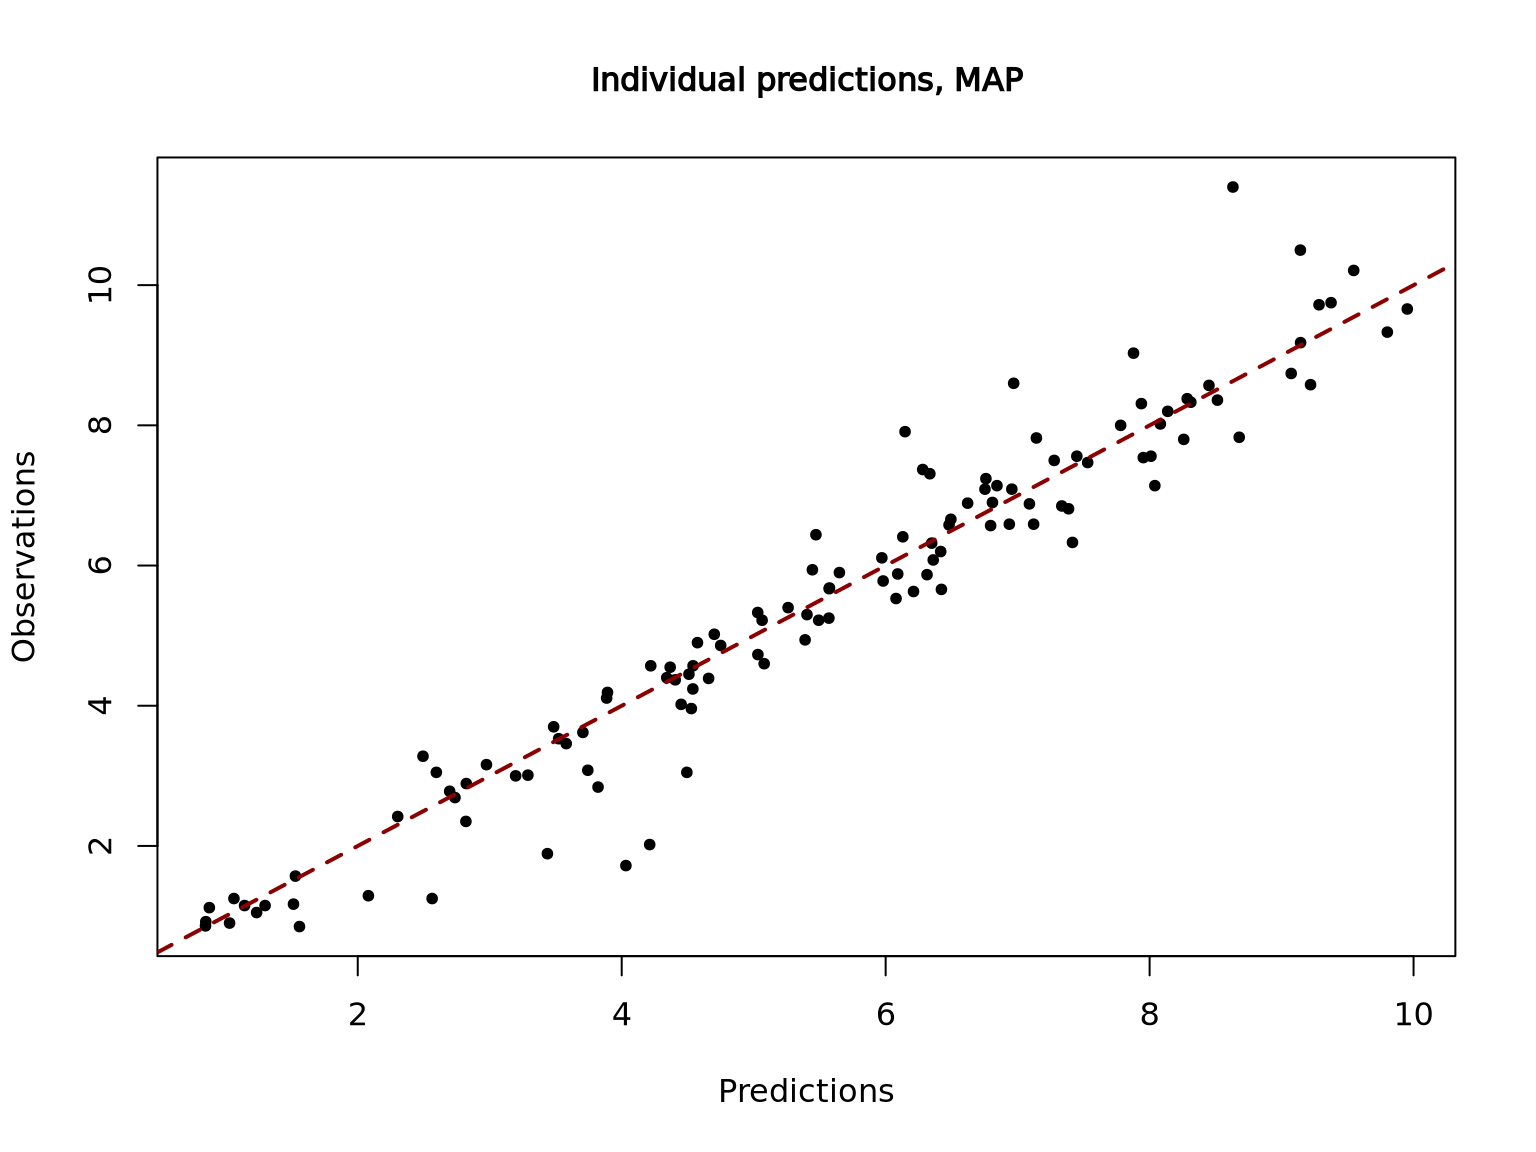
\includegraphics[width=0.8\textwidth]{nlme-fit}
    \caption{Fitted nonlinear mixed effects model showing population and individual responses.}
\end{figure}

\subsubsection{Example with Theophylline Data}
\paragraph{R Implementation:}
\begin{lstlisting}[language=R]
library(nlme)
pharm_model <- function(dose, ka, ke, cl) {
  return(dose * ka / (cl * (ka - ke)) * (exp(-ke*t)-exp(-ka*t)))
}
nlme_model <- nlme(conc ~ pharm_model(dose, ka, ke, cl),
                   data = Theoph,
                   fixed = ka + ke + cl ~ 1,
                   random = ka + ke + cl ~ 1 | Subject,
                   start = c(ka = 1.5, ke = 0.08, cl = 0.04))
library(saemix)
model_nlme <- function(psi, id, x) {
  D <- 320
  t <- x[,1]
  ka <- psi[id,1]
  V <- psi[id,2]
  ke <- psi[id,3]
  Dka/(V(ka-ke))(exp(-ket)-exp(-kat))
}
saemix_model <- saemixModel(
  model = modelnlme,
  psi0 = c(ka=1, V=20, ke=0.5)
)
\end{lstlisting}

\subsubsection{Extended Features}
\paragraph{1. Residual Error Models:}
\begin{itemize}
  \item Constant: $\varepsilon_{ij} \sim N(0, a^2)$
  \item Proportional: $\varepsilon_{ij} = b \cdot f(t_{ij}, \psi_i) \cdot \varepsilon_{ij}^*$, $\varepsilon_{ij}^* \sim N(0, 1)$
  \item Combined: $\varepsilon_{ij} = (a + b \cdot f(t_{ij}, \psi_i)) \cdot \varepsilon_{ij}^*$
\end{itemize}
\paragraph{2. Parameter Transformations:}
\begin{itemize}
  \item Log-normal: $\log(\psi_i) = \log(\psi_{\text{pop}}) + \eta_i$
  \item Logit-normal: $\text{logit}(\psi_i) = \text{logit}(\psi_{\text{pop}}) + \eta_i$
\end{itemize}
\paragraph{3. Covariate Models:}
\begin{lstlisting}[language=R]
# Volume depends on weight
covariate.model = c(0, 1, 0)
# Relationship: Vi = V{pop} * (WTi / WT{ref})^{beta_wt}
\end{lstlisting}
\paragraph{4. Correlations between Random Effects:}
\begin{lstlisting}[language=R]
covariance.model = matrix(c(1,1,1,1,1,1,1,1,1), nrow=3)
covariance.model = matrix(c(1,0,0,0,1,0,0,0,1), nrow=3)
covariance.model = matrix(c(1,1,0,1,1,0,0,0,1), nrow=3)
\end{lstlisting}

\begin{figure}[htb]
    \centering
    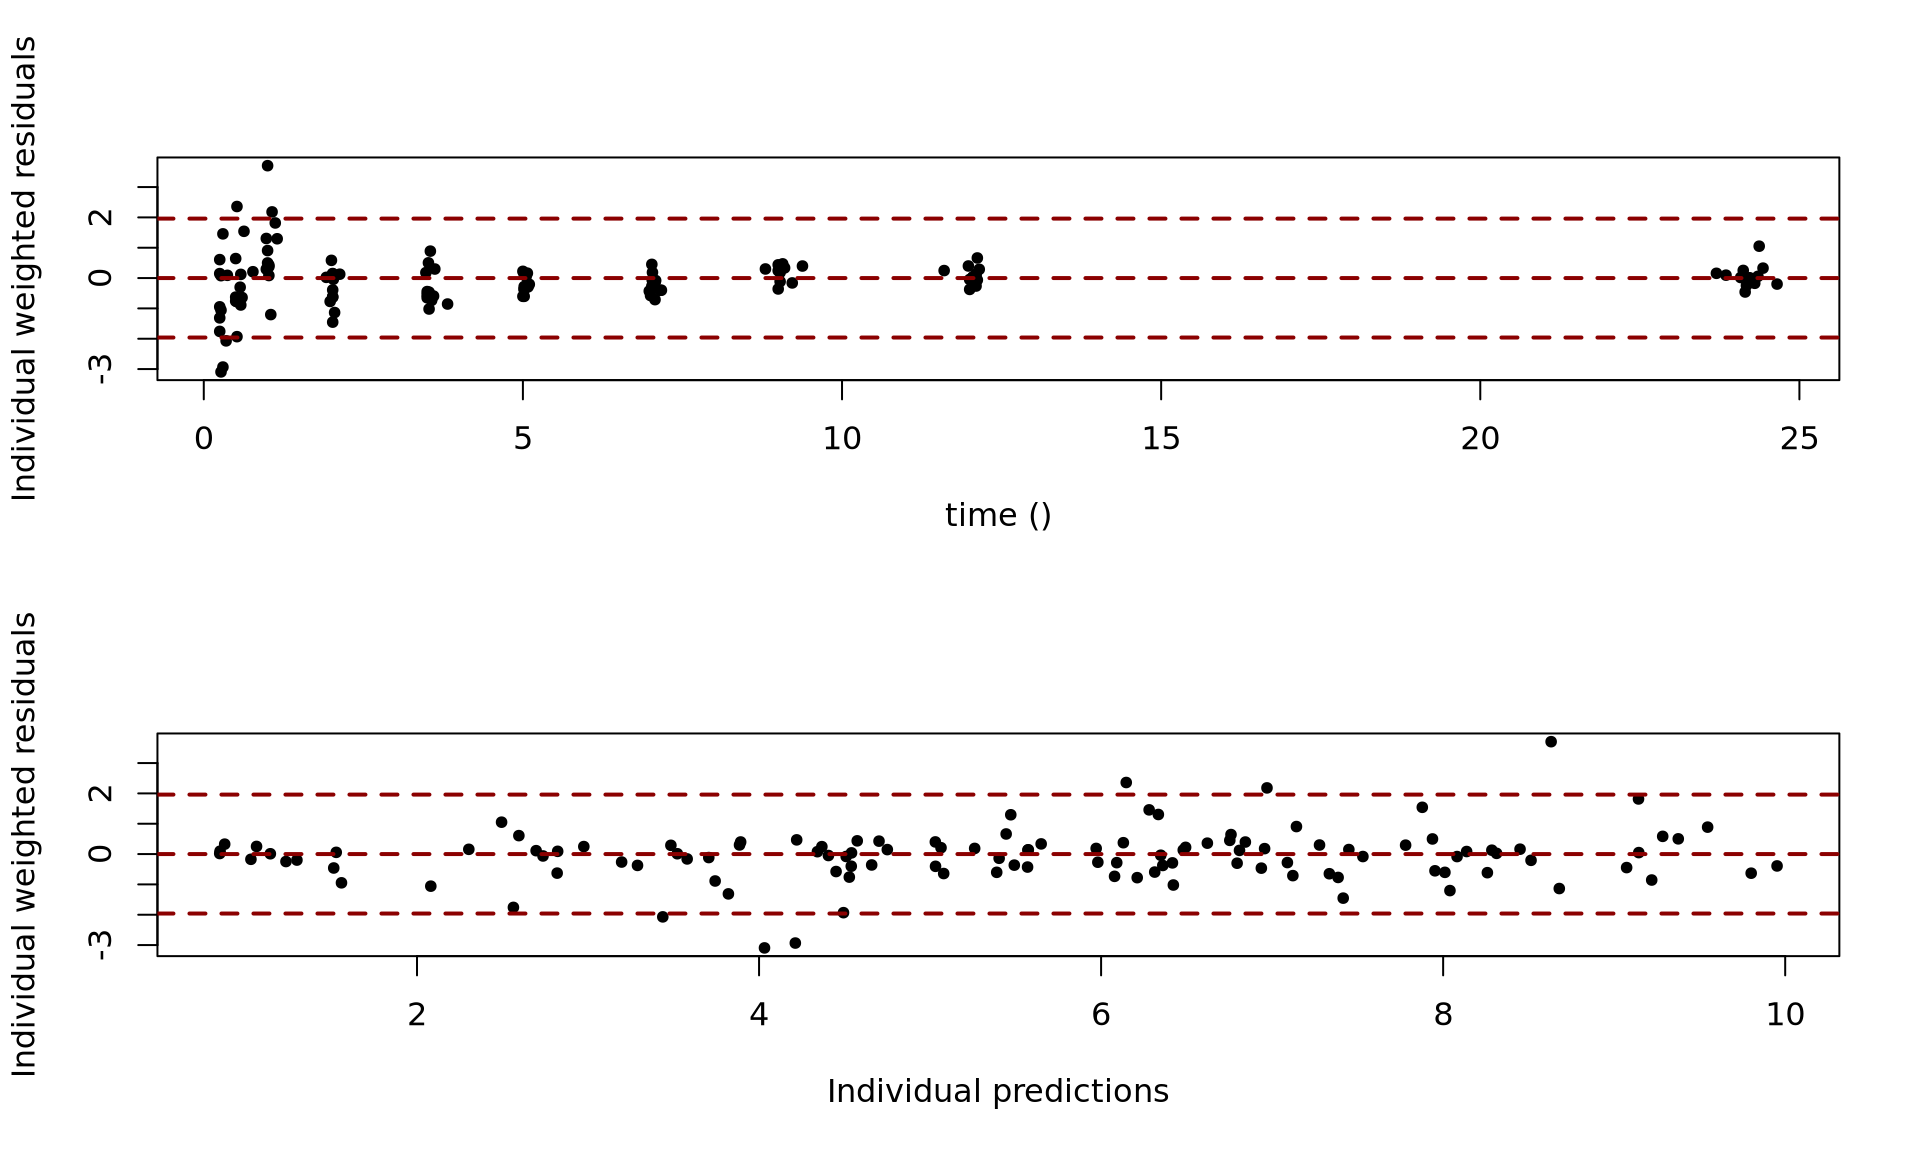
\includegraphics[width=0.8\textwidth]{nlme-diagnostics.png}
    \caption{Diagnostic plots for the NLME model.}
    \label{fig:nlme-diagnostics}
\end{figure}

Figure \ref{fig:nlme-diagnostics} presents diagnostics for the NLME model.

\newpage

\section{Mixture Models}

\subsection{Gaussian Mixture Models}

\subsubsection{Model Formulation}
For a K-component mixture:
\begin{equation}
p(x) = \sum_{k=1}^K \pi_k p_k(x|\theta_k)
\end{equation}
For Gaussian mixtures:
\begin{equation}
p(x) = \sum_{k=1}^K \pi_k \mathcal{N}(x|\mu_k, \Sigma_k)
\end{equation}

\begin{figure}[htb]
    \centering
    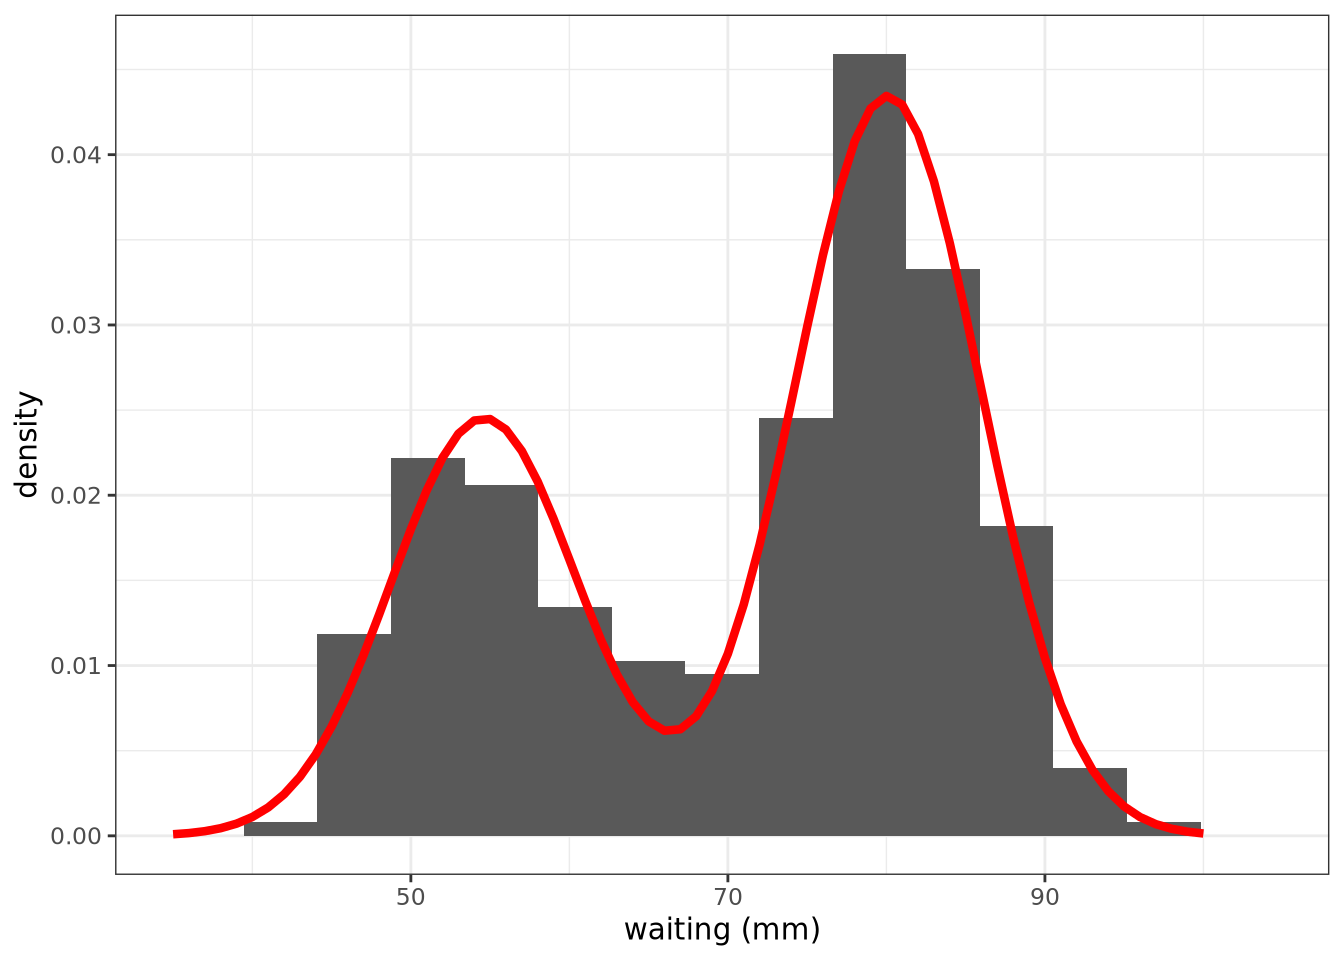
\includegraphics[width=0.8\textwidth]{mixture-density.png}
    \caption{Histogram with a mixture density fit for a bimodal distribution.}
    \label{fig:mixture-density}
\end{figure}

Figure \ref{fig:mixture-density} illustrates how component densities combine to form the overall density.

\subsubsection{Expectation-Maximization (EM) Algorithm}

\paragraph{E-step:} Compute responsibilities  
\[
\tau_{ik}^{(t)} = \frac{\pi_k^{(t)} \mathcal{N}(y_i|\mu_k^{(t)}, \sigma_k^{2,(t)})}{\sum_{j=1}^K \pi_j^{(t)} \mathcal{N}(y_i|\mu_j^{(t)}, \sigma_j^{2,(t)})}
\]
\paragraph{M-step:} Update parameters:
\begin{align}
\pi_k^{(t+1)} &= \frac{1}{n}\sum_{i=1}^n \tau_{ik}^{(t)} \\
\mu_k^{(t+1)} &= \frac{\sum_{i=1}^n \tau_{ik}^{(t)} y_i}{\sum_{i=1}^n \tau_{ik}^{(t)}} \\
\sigma_k^{2,(t+1)} &= \frac{\sum_{i=1}^n \tau_{ik}^{(t)} (y_i - \mu_k^{(t+1)})^2}{\sum_{i=1}^n \tau_{ik}^{(t)}}
\end{align}

\paragraph{R Implementation:}
\begin{lstlisting}[language=R]
mixture_gaussian1D <- function(x, K = 2, max_iter = 100, tol = 1e-6) {
  # Initialize parameters (e.g., using K-means)
  # Repeat until convergence:
  #   E-step: Calculate responsibilities
  #   M-step: Update parameters
  #   Calculate log-likelihood
  # Return parameters and cluster assignments
}

library(mixtools)
mixture_EM <- normalmixEM(faithful$waiting, k = 2)
summary(mixture_EM)
plot(mixture_EM, which = 2)

library(mclust)
mc <- Mclust(faithful$waiting)
summary(mc)
plot(mc, what = "density")
\end{lstlisting}

\begin{figure}[htb]
    \centering
    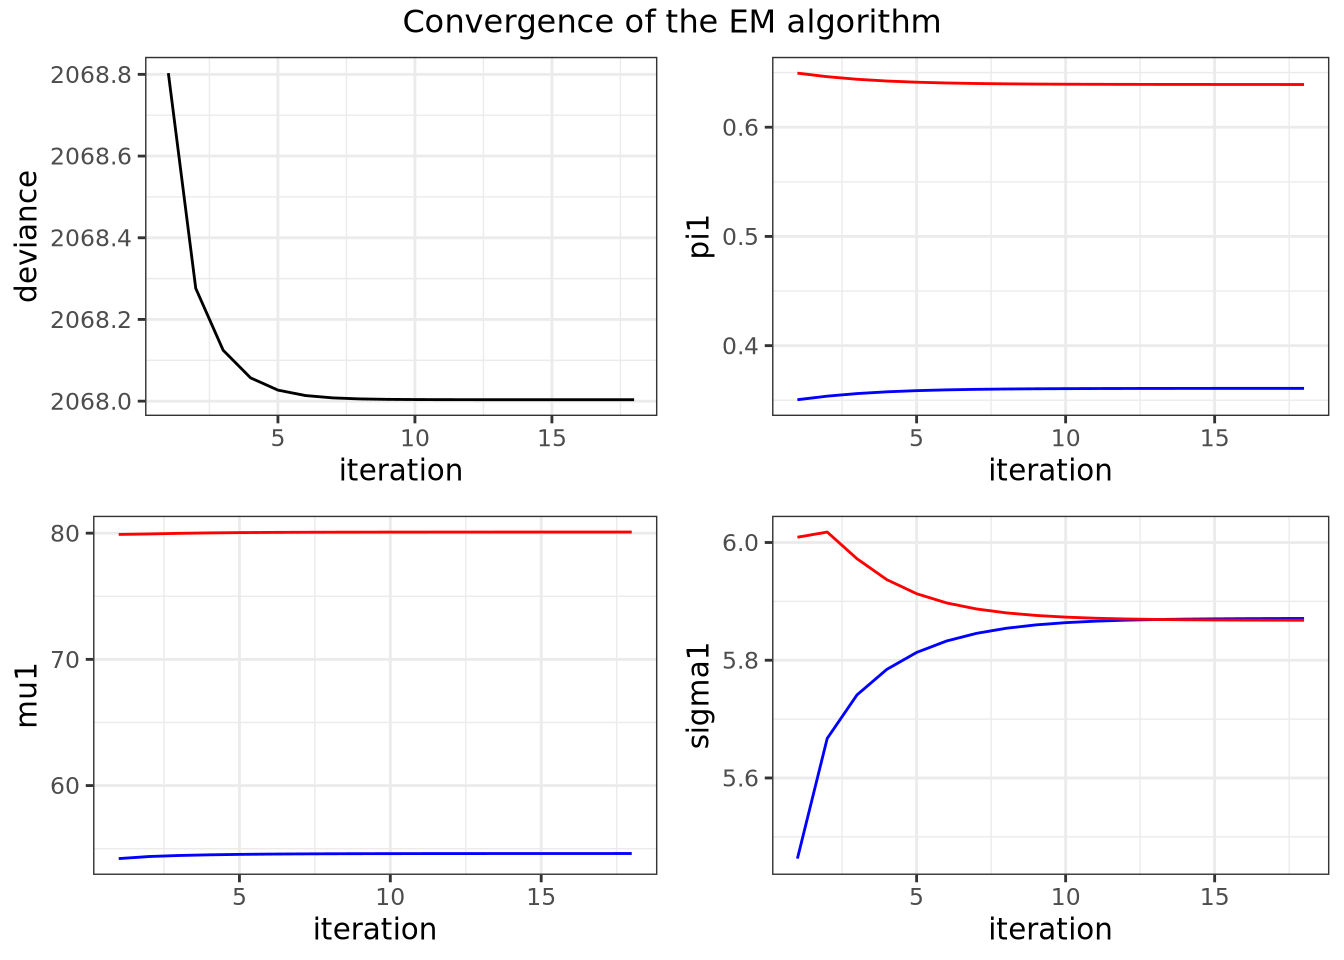
\includegraphics[width=0.8\textwidth]{em-convergence.png}
    \caption{EM algorithm convergence illustrating log-likelihood and parameter evolution.}
    \label{fig:em-convergence}
\end{figure}

Figure \ref{fig:em-convergence} demonstrates convergence over iterations.

\subsubsection{Non-identifiability Issue}
Label switching is inherent to mixture models. Possible solutions include:
\begin{itemize}
  \item Enforcing identifiability constraints (e.g., ordering by means)
  \item Using relabeling algorithms in Bayesian approaches
  \item Focusing on clustering results rather than component-specific parameters
\end{itemize}

\begin{warningbox}
Multiple initializations may yield different parameter estimates due to local optima and label switching.
\end{warningbox}

\subsection{Clustering and Classification}

\subsubsection{K-means Clustering}
\begin{equation}
U(\mu_1, \ldots, \mu_K) = \sum_{i=1}^n \min_{1 \le k \le K} ||y_i - \mu_k||^2
\end{equation}

\begin{figure}[htb]
    \centering
    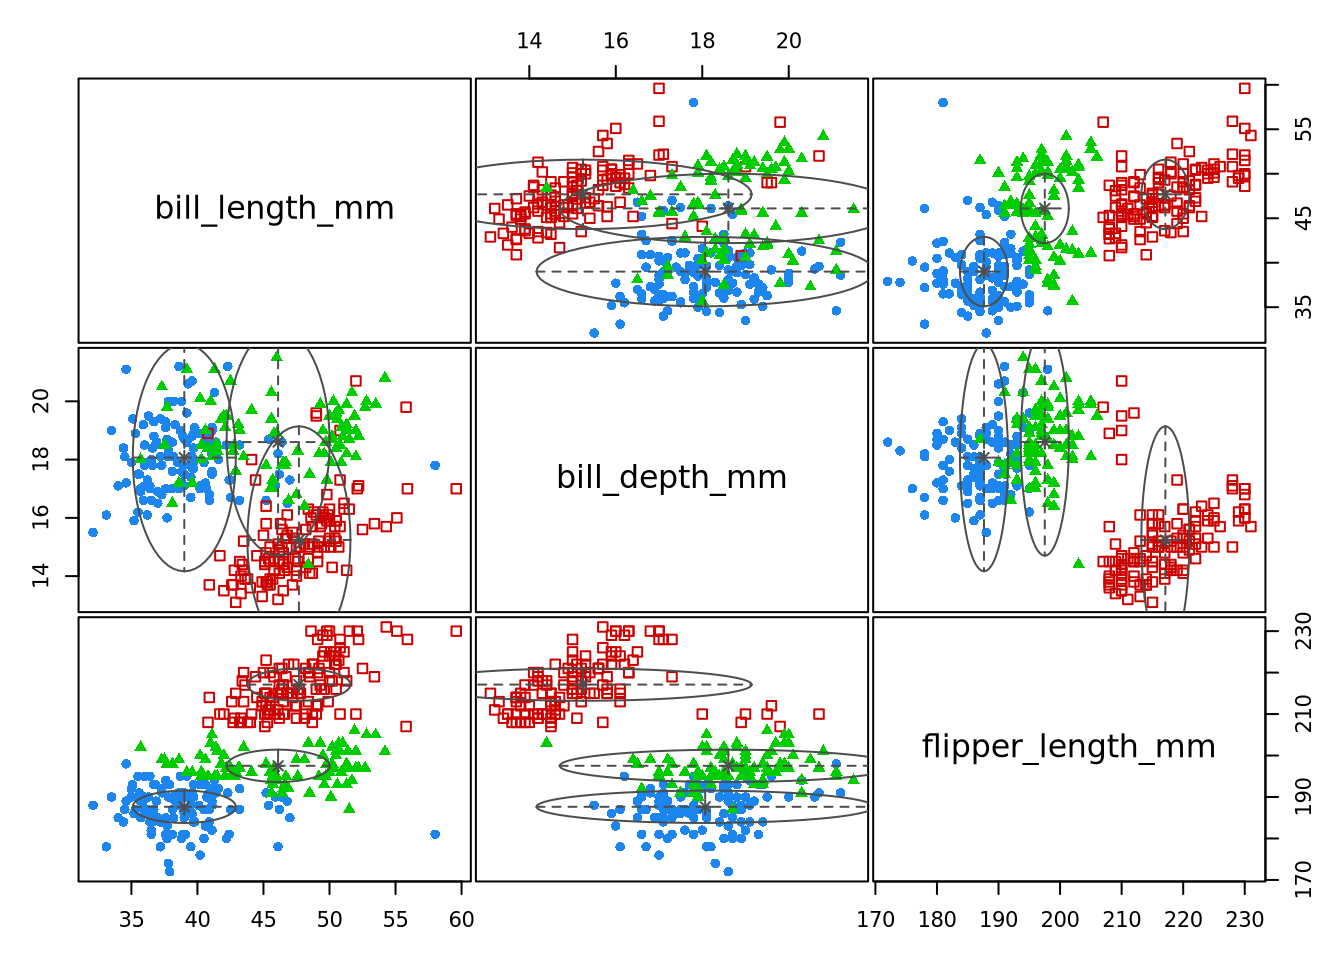
\includegraphics[width=0.8\textwidth]{kmeans-clustering.png}
    \caption{K-means clustering visualization in multiple dimensions.}
    \label{fig:kmeans}
\end{figure}

\paragraph{R Implementation:}
\begin{lstlisting}[language=R]
set.seed(123)
km <- kmeans(iris[, 1:4], centers = 3, nstart = 25)
table(km$cluster, iris$Species)
plot(iris[, 1:2], col = km$cluster, pch = 20)
wss <- sapply(1:10, function(k) {
  kmeans(iris[, 1:4], centers = k, nstart = 25)$tot.withinss
})
plot(1:10, wss, type = "b", xlab = "Number of clusters", ylab = "Within-cluster sum of squares")
\end{lstlisting}

\begin{tipbox}
K-means is fast and simple but assumes spherical clusters and may converge to local optima.
\end{tipbox}

\subsubsection{Supervised Classification}

\paragraph{Logistic Regression:}
\begin{equation}
\log\left(\frac{P(y_i = 1)}{1 - P(y_i = 1)}\right) = \beta_0 + \sum_{m=1}^M \beta_m c_{im}
\end{equation}

\paragraph{Multinomial Logistic Regression:}
\begin{equation}
\log\left(\frac{P(y_i = k)}{P(y_i = L)}\right) = \beta_{k0} + \sum_{m=1}^M \beta_{km}c_{im}
\end{equation}

\begin{figure}[htb]
    \centering
    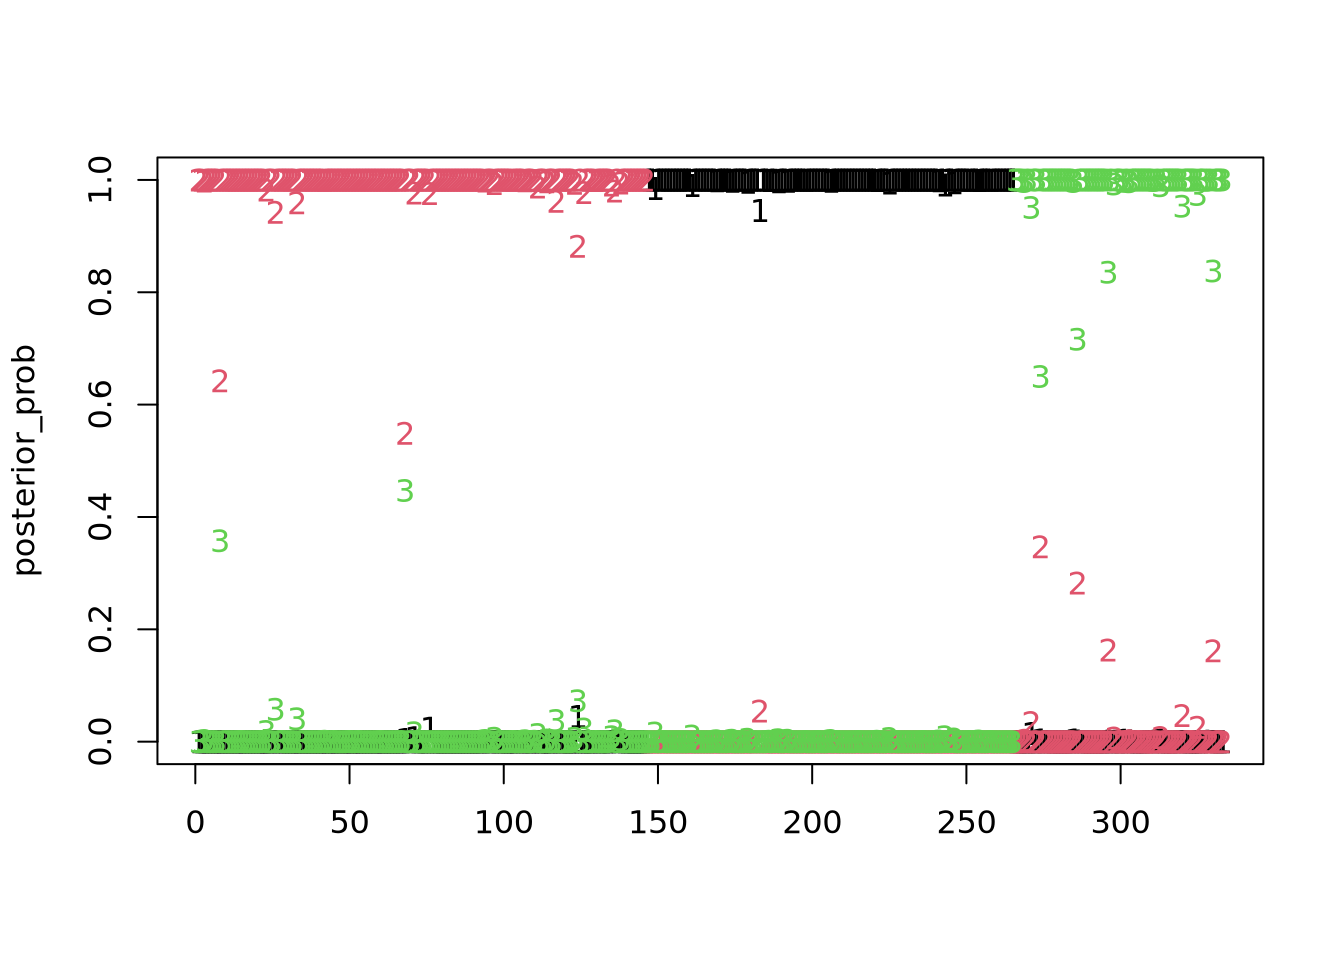
\includegraphics[width=0.8\textwidth]{classification-boundries.png}
    \caption{Classification plot with decision boundaries from multinomial logistic regression.}
    \label{fig:classification-boundaries}
\end{figure}

\paragraph{R Implementation:}
\begin{lstlisting}[language=R]
glm_bin <- glm(Species == "versicolor" ~ Sepal.Length + Petal.Width, data = iris, family = "binomial")
summary(glm_bin)
library(nnet)
multi <- multinom(Species ~ Sepal.Length + Petal.Width, data = iris)
summary(multi)
probs <- predict(multi, type = "probs")
preds <- predict(multi)
table(preds, iris$Species)
\end{lstlisting}

\subsubsection{Model-Based Clustering}
\begin{equation}
\hat{z}_i = \arg\max_k P(Z_i = k | y_i; \hat{\theta})
\end{equation}

\begin{figure}[htb]
    \centering
    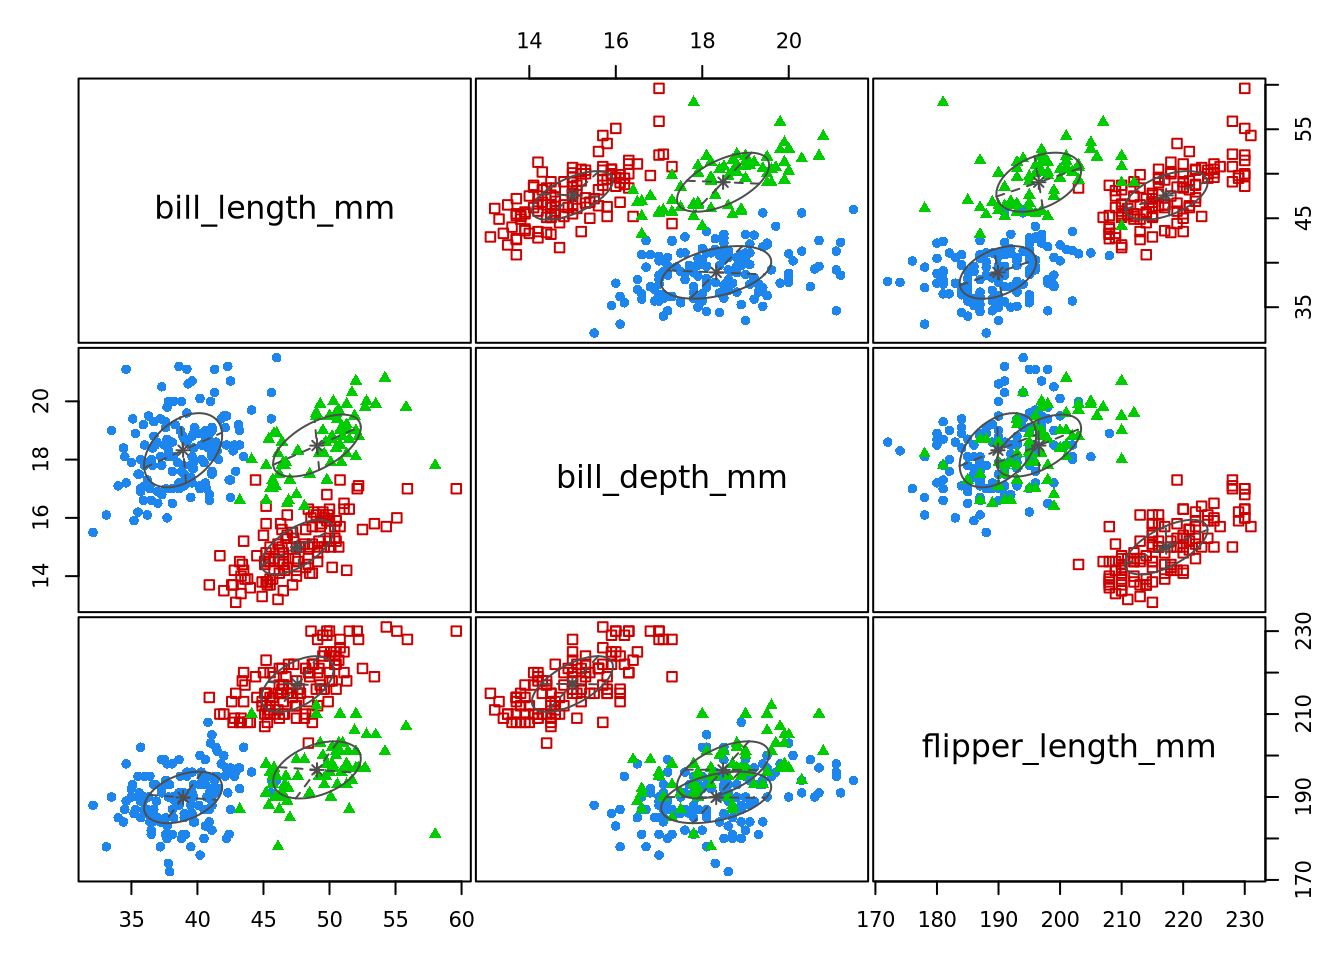
\includegraphics[width=0.8\textwidth]{model-based-clustering.png}
    \caption{Model-based clustering visualization with elliptical contours.}
    \label{fig:model-based-clustering}
\end{figure}
\begin{lstlisting}[language=R]
library(mclust)
GMM_best <- Mclust(penguins[, 2:4])
summary(GMM_best)
plot(GMM_best, what = "classification")
plot(GMM_best, what = "uncertainty")
probs <- GMM_best$z
class <- GMM_best$classification
\end{lstlisting}

\subsubsection{Evaluation Metrics}
\begin{lstlisting}[language=R]
library(aricode)
ARI(GMM_best$classification, penguins$species)
ARI(km$cluster, penguins$species)
NMI(GMM_best$classification, penguins$species)
AMI(GMM_best$classification, penguins$species)
\end{lstlisting}

\begin{notebox}
When true labels are not available, internal measures like the silhouette coefficient, BIC/AIC, or the gap statistic may be used.
\end{notebox}
\newpage

\section{Summary of Key Concepts}

\begin{mdframed}[linecolor=maincolor,backgroundcolor=gray!5!white]
\textbf{Hypothesis Testing}
\begin{itemize}
  \item Framework for decisions based on sampling distributions.
  \item Power analysis ensures sufficient sample size.
  \item Multiple testing corrections control false discoveries.
  \item P-values must be interpreted in context.
\end{itemize}
\end{mdframed}

\begin{mdframed}[linecolor=maincolor,backgroundcolor=gray!5!white]
\textbf{Regression Models}
\begin{itemize}
  \item Linear regression models relationships between variables.
  \item Start with simple models and validate assumptions.
  \item Consider transformations or nonlinear models as needed.
\end{itemize}
\end{mdframed}

\begin{mdframed}[linecolor=maincolor,backgroundcolor=gray!5!white]
\textbf{Mixed Models}
\begin{itemize}
  \item Analyze hierarchical or correlated data.
  \item Distinguish between fixed and random effects.
  \item Choose estimation methods (ML or REML) based on inference goals.
\end{itemize}
\end{mdframed}

\begin{mdframed}[linecolor=maincolor,backgroundcolor=gray!5!white]
\textbf{Mixture Models}
\begin{itemize}
  \item Useful for density estimation and clustering heterogeneous populations.
  \item EM algorithm is standard for parameter estimation.
  \item Address label switching and compare models using information criteria.
\end{itemize}
\end{mdframed}

\begin{mdframed}[linecolor=tipcolor!75!black,backgroundcolor=tipcolor!5!white]
\textbf{Statistical Computing in R}
\begin{itemize}
  \item R offers extensive tools for statistical analysis.
  \item Key packages include \texttt{stats}, \texttt{lme4}, \texttt{nlme}, and \texttt{mclust}.
  \item Effective visualization and model diagnostics are crucial.
\end{itemize}
\end{mdframed}

\begin{mdframed}[linecolor=warningcolor!75!black,backgroundcolor=warningcolor!5!white]
\textbf{Common Pitfalls to Avoid}
\begin{itemize}
  \item Not checking model assumptions.
  \item Ignoring multiple testing corrections.
  \item Overfitting by adding excessive complexity.
  \item Misinterpreting statistical significance.
\end{itemize}
\end{mdframed}

\begin{mdframed}[linecolor=maincolor,backgroundcolor=gray!5!white]
\textbf{Practical Guidelines for Real-World Application}
\begin{itemize}
  \item Start with exploratory data analysis.
  \item Document analysis decisions.
  \item Validate models with independent test data.
  \item Report uncertainty and limitations.
\end{itemize}
\end{mdframed}

\end{document}
